%%%%%%%%%%%%%%%%%%%%%%%%%%%%%%%%%%%%%%%%%%%%%%%%%%%%%%%%%%%%%%%%%%%%%
% LaTeX Template: Project Titlepage Modified (v 0.1) by rcx
%
% Original Source: http://www.howtotex.com
% Date: February 2014
% 
% This is a title page template which be used for articles & reports.
% 
% This is the modified version of the original Latex template from
% aforementioned website.
% 
%%%%%%%%%%%%%%%%%%%%%%%%%%%%%%%%%%%%%%%%%%%%%%%%%%%%%%%%%%%%%%%%%%%%%%

\documentclass[french, 12pt, a4paper, oneside]{report}
\usepackage{babel}
\usepackage[a4paper]{geometry}
%\usepackage[myheadings]{fullpage}
\usepackage{fancyhdr}
\usepackage{lastpage}
%\usepackage{graphicx, wrapfig, subcaption, setspace, booktabs}
\usepackage{setspace}
%\usepackage[T1]{fontenc}
%\usepackage[font=small, labelfont=bf]{caption}
%\usepackage{fourier}
%\usepackage[protrusion=true, expansion=true]{microtype}
%\usepackage{sectsty}
\usepackage[hyphens]{url}
\usepackage[hidelinks]{hyperref} 
\usepackage{tabularx}
\usepackage{tabulary}
\usepackage{multirow}
\usepackage{array}
\usepackage{caption, booktabs, makecell}
\usepackage{enumitem}
\usepackage{graphicx}
\usepackage{amsmath}
\usepackage[linesnumbered, french,ruled,vlined]{algorithm2e}
\usepackage{placeins}
\usepackage{listings}
\usepackage{forest}
\usepackage{titling}

\usepackage{tikz}
\usetikzlibrary{matrix,chains,positioning,decorations.pathreplacing,arrows}

\frenchbsetup{StandardLists=true}	% Permet d'utiliser des puces standards pour les item


\newcommand{\HRule}[1]{\rule{\linewidth}{#1}}
%\onehalfspacing
%\setcounter{tocdepth}{5}
%\setcounter{secnumdepth}{5}

\graphicspath{ {images/} }  %charger dossier d'images 

\usepackage[T1]{fontenc} % Pour l'encodage du français


\lstset{literate=
  {á}{{\'a}}1 {é}{{\'e}}1 {í}{{\'i}}1 {ó}{{\'o}}1 {ú}{{\'u}}1
  {Á}{{\'A}}1 {É}{{\'E}}1 {Í}{{\'I}}1 {Ó}{{\'O}}1 {Ú}{{\'U}}1
  {à}{{\`a}}1 {è}{{\`e}}1 {ì}{{\`i}}1 {ò}{{\`o}}1 {ù}{{\`u}}1
  {À}{{\`A}}1 {È}{{\'E}}1 {Ì}{{\`I}}1 {Ò}{{\`O}}1 {Ù}{{\`U}}1
  {ä}{{\"a}}1 {ë}{{\"e}}1 {ï}{{\"i}}1 {ö}{{\"o}}1 {ü}{{\"u}}1
  {Ä}{{\"A}}1 {Ë}{{\"E}}1 {Ï}{{\"I}}1 {Ö}{{\"O}}1 {Ü}{{\"U}}1
  {â}{{\^a}}1 {ê}{{\^e}}1 {î}{{\^i}}1 {ô}{{\^o}}1 {û}{{\^u}}1
  {Â}{{\^A}}1 {Ê}{{\^E}}1 {Î}{{\^I}}1 {Ô}{{\^O}}1 {Û}{{\^U}}1
  {Ã}{{\~A}}1 {ã}{{\~a}}1 {Õ}{{\~O}}1 {õ}{{\~o}}1
  {œ}{{\oe}}1 {Œ}{{\OE}}1 {æ}{{\ae}}1 {Æ}{{\AE}}1 {ß}{{\ss}}1
  {ű}{{\H{u}}}1 {Ű}{{\H{U}}}1 {ő}{{\H{o}}}1 {Ő}{{\H{O}}}1
  {ç}{{\c c}}1 {Ç}{{\c C}}1 {ø}{{\o}}1 {å}{{\r a}}1 {Å}{{\r A}}1
  {€}{{\euro}}1 {£}{{\pounds}}1 {«}{{\guillemotleft}}1
  {»}{{\guillemotright}}1 {ñ}{{\~n}}1 {Ñ}{{\~N}}1 {¿}{{?`}}1
}
%-------------------------------------------------------------------------------
% HEADER & FOOTER
%-------------------------------------------------------------------------------

\setlength{\headheight}{15pt}

\pagestyle{fancy}

\renewcommand{\chaptermark}[1]{ \markboth{#1}{} }
\renewcommand{\sectionmark}[1]{ \markright{#1} }


\fancyhf{}
\fancyhead[R]{\leftmark}
\fancyfoot[L]{\small{Alexis Plaquet, Tom Rivero}}
\fancyfoot[R]{Page \thepage\ / \pageref{LastPage}}

\fancypagestyle{plain}{
    \fancyhf{}%
    \fancyfoot[L]{\small{Alexis Plaquet, Tom Rivero}}
    \fancyfoot[R]{Page \thepage\ / \pageref{LastPage}}
    \renewcommand{\headrulewidth}{0pt}% Line at the header invisible
}

\renewcommand{\headrulewidth}{2pt}
\renewcommand{\footrulewidth}{1pt}

% Image UPJV sur la page de titre

% set up \maketitle to accept a new item
\predate{\begin{center}\placetitlepicture\large}
\postdate{\par\end{center}}

% commands for including the picture
\newcommand{\titlepicture}[2][]{%
  \renewcommand\placetitlepicture{%
    \includegraphics[#1]{#2}\par\medskip
  }%
}
\newcommand{\placetitlepicture}{} % initialization

%-------------------------------------------------------------------------------
% TITLE PAGE
%-------------------------------------------------------------------------------

\begin{document}

\title{ \normalsize \textsc{UE Projet}
		\\ [2.0cm]
		\HRule{0.5pt} \\
		\Large \textbf{\uppercase{Apprentissage par renforcement \\Rapport final}}
		\HRule{2pt} \\ [0.5cm]
		\normalsize \today \vspace*{5\baselineskip}}

\date{}

\author{
		Alexis Plaquet, Tom Rivero \\\\
		\small{Université Picardie Jules Verne} }

\titlepicture[width=3cm]{logo-UPJV.png}

\maketitle


\newpage
\thispagestyle{empty}
\null\newpage

%-------------------------------------------------------------------------------
% Section title formatting
%\sectionfont{\scshape}
%-------------------------------------------------------------------------------

%-------------------------------------------------------------------------------
% INTRODUCTION
%-------------------------------------------------------------------------------

%\chapter*{Introduction}


%-------------------------------------------------------------------------------
% TABLE DES MATIERES
%-------------------------------------------------------------------------------

\tableofcontents
\newpage

%-------------------------------------------------------------------------------
% BODY
%-------------------------------------------------------------------------------
\thispagestyle{fancy}


\chapter*{Introduction}
Vous trouverez dans ce document le rapport détaillé du travail du binôme Alexis Plaquet, Tom Rivero sur l'apprentissage par renforcement. Sont intégrées dans ce document toutes les parties présentes dans le cahier des charges, corrigées en prenant compte les conseils du professeur référent Mme Yu Li.


\chapter{Besoins et objectifs}

\section{Origine du besoin}

L'objectif de ce projet est de développer un programme d’apprentissage par renforcement capable de jouer à un jeu, dans le cadre de l’UE Projet de L3 informatique. 
\par
Le choix du jeu en question ainsi que des algorithmes utilisés reste libre, cependant l'énoncé original du sujet mentionnait Pac-Man ainsi que Space Invaders comme jeux possibles (modifié depuis pour n'inclure que la recherche de trésor et le Tic-tac-toe). Ces exemples de jeux ont éveillé notre curiosité sur le sujet, et nous avons donc décidé de tenter d'appliquer l'apprentissage par renforcement sur Pac-Man, qui est un jeu relativement complexe.
\par
Toutefois suite aux conseils du professeur référent et aux recherches de solutions à ce problème, nous avons pris conscience de la difficulté du projet. Nous avons en conséquence décidé d'appliquer dans un premier temps l'apprentissage par renforcement sur la recherche de trésor, un jeu extrêmement basique, afin d'en acquérir les bases et les concepts. Une fois cette étape franchie, nous pourrions nous attarder sur le plus complexe : Pac-Man.

\section{Principe du jeu ``Recherche de trésor''}

Le jeu “Recherche de trésor” est un jeu simple où il est possible de déplacer case par case un personnage dans un espace en une ou deux dimensions, et dont le but est d’arriver jusqu’à un trésor. En deux dimensions, il est aussi possible d’ajouter des murs et des obstacles afin de complexifier la tâche. 
\par
Ce jeu ne possède aucune difficulté particulière, spécialement en une dimension où le personnage n'a qu'à avancer à répétition dans la bonne direction jusqu'au trésor.
\par
En deux dimensions, l'agent devra mémoriser le chemin à emprunter pour arriver jusqu'au trésor.

\section{Principe de Pac-Man}
Pac-Man est un jeu d’arcade sorti en 1980 où l’on dirige le personnage éponyme dans un labyrinthe rempli d’objets à ramasser, l’objectif étant de ramasser toutes les “pac-gommes” pour passer au niveau suivant.
Pour complexifier la tâche, 4 fantômes rôdent dans le labyrinthe, et font perdre une vie à Pac-Man (qui en possède 3) au moindre contact . Il est temporairement possible de pouvoir les éliminer en ramassant certains objets, mais les fantômes finiront par réapparaître.
\par
Chacun des 4 fantômes a un comportement différent :

\begin{itemize}
	\item Le rouge suit Pac-Man à la trace
	\item Le rose et le bleu essayent de couper la route à Pac-Man en se plaçant devant lui
	\item Le orange se déplace aléatoirement
\end{itemize}


\section{Principe de l’apprentissage par renforcement}

L’apprentissage par renforcement est une méthode d’apprentissage où un \textbf{agent} logiciel autonome doit apprendre quelles actions effectuer dans un \textbf{environnement} donné, de façon à obtenir la plus grande récompense possible.\par

Ce genre d’algorithme fonctionne généralement à l’aide de 3 entités : 
\begin{itemize}
	\item Un agent, qui va prendre les décisions et effectuer des actions
	\item Un environnement, sur lequel l’agent agira
	\item Une interface, qui se chargera de fournir les informations actuelles sur l’environnement à l’agent (image, son, données numériques, etc) ainsi que la ``récompense'' associée à chaque action effectuée.
\end{itemize}

On désigne par récompense une valeur numérique arbitraire indiquant la qualité de l'action effectuée. Une récompense positive est associée à un comportement désiré menant à la victoire (augmenter le score, avancer dans le niveau, se rapprocher d'un objet, etc), tandis qu'une récompense négative est associée à un comportement néfaste à l'objectif visé (perdre une vie, prendre des dégats, etc).
Ici, l’environnement sera un jeu Pac-Man standard, et l’agent se substituera au joueur pour y jouer.


\section{Moyens et contraintes}
\subsection{Moyens financiers}
Le cadre dans lequel nous réalisons ce projet ne permet pas d’obtenir un budget pour son développement. Toutefois, ce dernier ne devrait pas nécessiter de dépense, et s’appuiera sur des technologies et ressources libres de droit.

\subsection{Moyens humains}
L’unique équipe derrière ce produit est constitué du binôme d’étudiants en charge du projet (Alexis PLAQUET et Tom RIVERO). Il est cependant possible d’obtenir de l’aide et des renseignements auprès des professeurs chargés d’assurer l’UE Projet.

\section{Modalités de mise en oeuvre}
Le client requiert seulement que le programme soit utilisable sous Linux.



\chapter{Analyse de l’existant, concurrence et positionnement}

\section{Description de l’existant}
Ce projet n’a pas pour objectif d’être novateur, il est en effet courant de tester des algorithmes d’apprentissage par renforcement sur des jeux vidéos, notamment parce que ces derniers sont facilement compréhensible pour les humains, que la lecture de l’écran de jeu est plus simple et intéressante qu’avec des jeux plus théoriques, et qu’il est aisé de comparer les performances d’une intelligence artificielle à celles d’un humain.

\section{Analyse de l’existant}
\subsection{Maluuba}
Le projet de faire jouer une intelligence artificielle à Pac-Man a été complètement accompli en 2017 par Maluuba \cite{maluuba}.
Maluuba a développé un agent utilisant utilise des techniques bien au delà des moyens de ce projet, comme la Hybrid Reward Architecture, afin d'atteindre le score maximal possible sur Pac-Man \cite{hra}.

\subsection{Projets amateurs}
De par la popularité d'OpenAI Gym, une librairie offrant de nombreux environnements (dont des jeux), on retrouve évidemment des projets identiques au nôtre. Ces derniers sont souvent des projets amateurs, des projets universitaires, et des projets effectués dans le cadre de recherches. La grande majorité est d’excellente qualité et la plupart bien documentée \cite{pacmanai1,pacmanai2,pacmanai3}.


\section{Positionnement par rapport à l'existant}
Comme évoqué précédemment, les objectifs que nous nous sommes fixés ont déjà été accomplis par d’autres personnes, et il paraît peu réaliste d’imaginer un projet dans ce domaine et avec nos compétences actuelles qui serait novateur.
\par
Le but principal de ce projet est avant tout de nous permettre de comprendre et d’appliquer la théorie et les algorithmes derrière l’apprentissage par renforcement.

\section{Cible du produit}
Sont ciblées principalement les personnes intéressées par l’apprentissage par renforcement. Celles-ci devront être capable d’installer d’elles même les librairies ou logiciels nécessaire à l'exécution de l’algorithme. Bien que ce rapport soit en français, l'entièreté du code ainsi que ses commentaires seront en anglais afin de permettre sa compréhension au plus grand nombre.
\par
Enfin, il est à noter que ce projet ne fera pas l’objet d’efforts d’accessibilité, il sera donc probablement inutilisable pour un usager malvoyant par exemple.


\chapter{Offre fonctionnelle}
\section{Fonctions principales}
Le logiciel disposera de trois modes principaux : entraînement, visualisation et tests. \par

On pourra ainsi entraîner un agent choisi, c’est à dire le laisser en phase d’apprentissage afin qu’il améliore la prédiction des actions à effectuer et apprenne à jouer
\par
La visualisation permet de voir de façon graphique comment l’IA joue, on pourra contrôler la vitesse d’affichage du jeu (afficher le jeu en ralenti ou en accéléré).
\par
Enfin, le mode test permettra de lancer une série de simulations pour voir quel score l’IA obtient en moyenne, le pourcentage d'échec, ainsi que toute autre statistique utile permettant d’évaluer la qualité de l’IA actuelle.

\section{Fonctions optionnelles}
Bien que intéressantes et utiles dans le cadre du projet, ces fonctionnalités pourraient être coûteuses en temps d’implémentation. \par

Au démarrage du logiciel, l’utilisateur pourra sélectionner sur quel jeu ou simulation il souhaite faire travailler l’apprentissage par renforcement, il pourra alors choisir parmi une liste prédéterminée. \par
Une fois ceci fait, l’utilisateur pourra choisir avec quel type d’algorithme d’apprentissage par renforcement il souhaite travailler, puis si cela a un sens dans le contexte de l’algorithme, choisir les paramètres de ce dernier. A ce moment il sera aussi possible à l’utilisateur de choisir de charger une sauvegarde existante de l’IA entraînée s’il en existe. L’utilisateur pouvant sauvegarder son IA après chaque entraînement. \par
Il serait aussi possible à l’utilisateur de jouer lui-même au jeu qu’il a sélectionné, si cela est humainement possible (cela pourrait ne pas l’être dans le cadre de certaines simulations).
\par
Il est aussi envisageable d'ajouter une interface graphique permettant de contrôler le tout de façon plus intuitive et rapide.


\section{Description fonctionnelle}

%---Entrainer---
\begin{center}
\begin{tabularx}{\linewidth}{|p{2.8cm}|X|}
    \hline
	\multicolumn{2}{|c|}{\textbf{Entrainer l'agent}}\\
	\hline
	\hline
	Description &
	Lance l'apprentissage de l'agent selon des paramètres donnés. \\
	\hline
	Paramètres d'entrée &
	\begin{minipage}[t]{\linewidth}
    \begin{itemize}[nosep,after=\strut,leftmargin=*]
        \item Nombre d'épisodes
        \item Affichage ou non des informations au fil de l'entraînement
        \item Paramètres spécifiques à chaque type d’algorithme d’apprentissage par renforcement
    \end{itemize}
    \end{minipage}
    \\ 
	\hline
	Paramètres de sortie &
	La structure de donnée de l'agent une fois entraîné\\
	\hline
	Contraintes à vérifier avant l'exécution &
	Le nombre d'épisode doit être un entier strictement positif \\
	\hline
	En cas d'erreur &
	Arrêter l'entraînement et en informer l’utilisateur \\
	\hline
	Priorité &
	Must \\
	\hline
\end{tabularx}
\end{center}

\vspace*{1 cm}

%---Tester---
\begin{center}
\begin{tabulary}{1.0\textwidth}{|L | L |}
	\hline
	\multicolumn{2}{|c|}{\textbf{Tester l'agent}}\\
	\hline
	\hline
	Description &
	Laisse l'agent compléter un nombre d’épisodes donné et calcule les statistiques de victoire, la moyenne d’actions nécessaires pour gagner une partie, etc\\
	\hline
	Paramètres d'entrée &
	\begin{minipage}[t]{\linewidth}
    \begin{itemize}[nosep,after=\strut,leftmargin=*]
        \item Nombre d'épisodes
    \end{itemize}
    \end{minipage}
    \\
	\hline
	Paramètres de sortie &
	Les données et statistiques résultant des tests\\
	\hline
	Contraintes à vérifier avant l'exécution &
	Le nombre d’épisodes doit être un entier strictement positif \\
	\hline
	En cas d'erreur &
	Arrêter le test, en informer l’utilisateur \\
	\hline
	Priorité &
	Must \\
	\hline
\end{tabulary}
\end{center}

\vspace*{1 cm}

%---Regarder jouer---

\begin{center}
  \begin{tabularx}{\linewidth}{|p{2.8cm}|X|}
    \hline
	\multicolumn{2}{|c|}{\textbf{Regarder l’agent jouer}}\\
	\hline
	\hline
	Description &
	Lance la visualisation graphique de l’agent jouant en temps réel\\
	\hline
	Paramètres d'entrée &
	\begin{minipage}[t]{\linewidth}
    \begin{itemize}[nosep,after=\strut,leftmargin=*]
        \item Vitesse de lecture
        \item Nombre de parties
    \end{itemize}
    \end{minipage}
    \\ 
	\hline
	Paramètres de sortie &
	Affichage graphique du jeu\\
	\hline
	Contraintes à vérifier avant l'exécution &
	La vitesse de lecture doit être un réel strictement positif et le nombre d’épisodes doit être un entier strictement positif \\
	\hline
	En cas d'erreur &
	Arrêter la lecture, en informer l’utilisateur \\
	\hline
	Priorité &
	Should \\
	\hline
  \end{tabularx}
\end{center}

\vspace*{1 cm}

%---Sauvegarder---

\begin{center}
  \begin{tabularx}{\linewidth}{|p{2.8cm}|X|}
    \hline
	\multicolumn{2}{|c|}{\textbf{Sauvegarder l'agent}}\\
	\hline
	\hline
	Description &
	Permet de sauvegarder l’état actuel de l’IA utilisée\\
	\hline
	Paramètres d'entrée &
	\begin{minipage}[t]{\linewidth}
    \begin{itemize}[nosep,after=\strut,leftmargin=*]
        \item Nom du fichier
    \end{itemize}
    \end{minipage}
    \\ 
	\hline
	Paramètres de sortie &
	Le fichier sauvegardé\\
	\hline
	Contraintes à vérifier avant l'exécution &
	Avoir les droits d’écriture sur le nom du fichier donné \\
	\hline
	En cas d'erreur &
	Informer l’utilisateur que le fichier n’a pas pu être sauvegardé \\
	\hline
	Priorité &
	Should \\
	\hline
  \end{tabularx}
\end{center}

\vspace*{1 cm}

%---Charger---

\begin{center}
  \begin{tabularx}{\linewidth}{|p{2.8cm}|X|}
    \hline
	\multicolumn{2}{|c|}{\textbf{Charger l'agent}}\\
	\hline
	\hline
	Description &
	Permet de charger depuis le disque dur une IA précédemment sauvegardée\\
	\hline
	Paramètres d'entrée &
	\begin{minipage}[t]{\linewidth}
    \begin{itemize}[nosep,after=\strut,leftmargin=*]
        \item Nom du fichier
    \end{itemize}
    \end{minipage}
    \\ 
	\hline
	Paramètres de sortie &
	L’IA chargée\\
	\hline
	Contraintes à vérifier avant l'exécution &
	Avoir les droits de lecture sur le nom du fichier donné \\
	\hline
	En cas d'erreur &
	Informer l’utilisateur que le fichier n’a pas pu être chargé \\
	\hline
	Priorité &
	Should \\
	\hline
  \end{tabularx}
\end{center}

\vspace*{1 cm}


%---Selectionner jeu---

\begin{center}
  \begin{tabularx}{\linewidth}{|p{2.8cm}|X|}
    \hline
	\multicolumn{2}{|c|}{\textbf{Sélectionner l'environnement}}\\
	\hline
	\hline
	Description &
	Permet de sélectionner le jeu ou la simulation sur laquelle on souhaite faire travailler l’IA\\
	\hline
	Paramètres d'entrée &
	\begin{minipage}[t]{\linewidth}
    \begin{itemize}[nosep,after=\strut,leftmargin=*]
        \item Nom du jeu
    \end{itemize}
    \end{minipage}
    \\ 
	\hline
	Paramètres de sortie &
	\\
	\hline
	Contraintes à vérifier avant l'exécution &
	Le jeu doit exister dans la base de données \\
	\hline
	En cas d'erreur &
    Informer l’utilisateur que le jeu n’est pas valide ou qu’une erreur s’est produite lors de son chargement \\
	\hline
	Priorité &
	Could \\
	\hline
  \end{tabularx}
\end{center}

\vspace*{1 cm}

%---Selectionner jeu---

\begin{center}
  \begin{tabularx}{\linewidth}{|p{2.8cm}|X|}
    \hline
	\multicolumn{2}{|c|}{\textbf{Sélectionner un type d’algorithme d’apprentissage par renforcement
}}\\
	\hline
	\hline
	Description &
	Permet de sélectionner un type d’algorithme avec lequel travailler\\
	\hline
	Paramètres d'entrée &
	\begin{minipage}[t]{\linewidth}
    \begin{itemize}[nosep,after=\strut,leftmargin=*]
        \item Le type d’algorithme
        \item Les paramètres requis par l’algorithme
    \end{itemize}
    \end{minipage}
    \\ 
	\hline
	Paramètres de sortie &
	Un agent de l’algorithme demandé
	\\
	\hline
	Contraintes à vérifier avant l'exécution &
	Le type d’algorithme doit exister et les paramètres doivent être valides \\
	\hline
	En cas d'erreur &
    Informer l’utilisateur que sa sélection est incorrecte
    \\
	\hline
	Priorité &
	Would \\
	\hline
  \end{tabularx}
\end{center}

%---Jouer au jeu---

\begin{center}
  \begin{tabularx}{\linewidth}{|p{2.8cm}|X|}
    \hline
	\multicolumn{2}{|c|}{\textbf{Laisser l'utilisateur jouer à l'environnement
}}\\
	\hline
	\hline
	Description &
	Permet de jouer manuellement au jeu ou à la simulation actuelle\\
	\hline
	Paramètres d'entrée & Jeu désiré
    \\ 
	\hline
	Paramètres de sortie &
	\\
	\hline
	Contraintes à vérifier avant l'exécution &
	Le jeu doit exister et pouvoir être jouable par un humain \\
	\hline
	En cas d'erreur &
    Informer l’utilisateur que sa sélection est incorrecte
    \\
	\hline
	Priorité &
	Would \\
	\hline
  \end{tabularx}
\end{center}

\chapter{Maquette et charte graphique}

L’IA sera exécutée depuis l’invite de commande, la seule interface graphique sera l’affichage du jeu.
Une charte graphique n'a donc pas lieu d'être.
L’utilisateur se verra présenter des menus à choix multiples ainsi que des entrées de textes afin de naviguer parmi les menus et définir les paramètres.
En voici des exemples permettant d’accéder aux différentes fonctionnalités précédemment introduites.

Au lancement du logiciel, l’utilisateur pourra choisir le type de jeu sur lequel travailler, puis une fois ce dernier choisi l’utilisateur devra choisir quel type d’apprentissage par renforcement il souhaite utiliser (il pourra aussi à ce moment choisir de jouer lui même au jeu)

\begin{center}
\includegraphics[width=0.5\textwidth]{maquette_choixjeu.png}
\includegraphics[width=0.5\textwidth]{maquette_choixia.png}
\end{center}

Dans le cas où le joueur choisit de charger une IA, la liste des IA précédemment sauvegardées sera affichée.

\begin{center}
\includegraphics[width=0.5\textwidth]{maquette_chargeria.png}
\end{center}

Une fois l’IA choisie ou chargée, l’utilisateur arrive sur le menu principal où il peut sélectionner une action à effectuer sur l’IA.

\begin{center}
\includegraphics[width=0.5\textwidth]{maquette_actionia.png}
\end{center}

Dans le cas où l’utilisateur souhaite entraîner l’IA, il devra entrer plusieurs paramètres permettant de configurer cet entraînement.

\begin{center}
\includegraphics[width=0.5\textwidth]{maquette_entraineria.png}
\end{center}

Une fois l'entraînement de l’IA terminé, l'utilisateur a la possibilité de sauvegarder l’IA entraînée pour la réutiliser ultérieurement.

\begin{center}
\includegraphics[width=0.5\textwidth]{maquette_sauvegarderia.png}
\end{center}

Enfin, si l’utilisateur désire voir l’IA jouer, il doit entrer quelques paramètres, et le jeu (joué par l’IA) sera affiché.

\begin{center}
\includegraphics[width=0.5\textwidth]{maquette_sauvegarderia.png}
\includegraphics[width=0.5\textwidth]{maquette_mspacman.png}
\end{center}


\chapter{Analyse du projet}
Du cahier des charges ressort deux objectifs principaux : en utilisant l'apprentissage par renforcement, faire tout d'abord jouer un agent à la recherche de trésor en utilisant le Q-Learning, puis réussir à faire jouer un agent à Pac-Man en utilisant le Deep Q-Learning.

\section{Contraintes}

La première partie du projet, c'est-à-dire la création d'un agent fonctionnant par Q-Learning et dans un environnement de recherche de trésor, ne pose pas de problème ou de contraintes particulière. En effet, l'algorithme de Q-Learning est relativement simple à implémenter et peut se faire dans n'importe quel langage de programmation. De même pour l'environnement de recherche de trésor qui ne consiste qu'au déplacement d'un joueur sur une grille en deux dimensions avec gestion des collisions.
\par
C'est la seconde partie qui va contraindre les choix possibles. Deux difficultés s'offrent à nous : la première est l'utilisation de réseaux de neurones, la deuxième est l'utilisation d'un environnement simulant PacMan.
\par
Bien qu'il soit tout à fait possible de développer soi-même une librairie simple pour gérer des réseaux de neurones, lors du développement du projet notre expérience dans le domaine était bien trop faible pour partir de zéro et arriver à des résultats concluant. Il était donc nécessaire de trouver un langage accueillant des librairies adaptées à l'apprentissage profond.
\par
De même, il est tout à fait possible de développer un jeu Pac-Man dans l'espace de temps donné pour le projet, cependant cette tâche représente un sujet de projet à elle seule, et il nous a paru irréaliste d'espérer pouvoir arriver à tenir cet objectif. Le langage choisi devra en conséquence posséder une librairie permettant de lier la librairie gérant les réseaux de neurones à un émulateur ou un jeu semblable à Pac-Man.
\par
Enfin, notons que le sujet mentionne que le programme final devra pouvoir être utilisé sous un environnement Linux.


\section{Analyse et choix de solutions}
\subsection{Choix du langage}
Le choix du langage importe relativement peu vis-à-vis de la contrainte majeure qu'est l'existence d'une librairie de machine learning. En effet, l'essor incroyable de ce domaine ces dernières années a pour conséquence la présence d'au moins une librairie de machine learning dans la plupart des langages. De plus dans notre cas la librairie choisie n'a pas besoin d'être à l'état de l'art, des fonctionnalités de bases suffisent amplement à accomplir nos objectifs. Nous avons donc restreint notre choix au langages que nous connaissions : Java, Python et C.
\par
Ce dernier est toutefois un langage très rigide où les tests rapides et les itérations de développements ne sont pas aisés.
Et bien qu'il soit très performant, c'est majoritairement la librairie de machine learning qui définira la performance du programme. Nous avons donc décidé de privilégier le Java ou le Python, tous deux bien plus souples et simples à utiliser.
\par
Le Java et le Python sont utilisés en machine learning, mais depuis quelques années c'est surtout Python qui s'est imposé comme un des langage de prédilection du machine learning avec le langage R. De nombreuses librairies de très bonne qualité possèdent des bindings en Python, et un grand nombre de ressources sont disponibles en ligne (tutoriels, exemples). Le Python est aussi un langage à la syntaxe très simple et souple (non typé, utilisant le duck-typing), au prix d'une performance plus faible (toutefois en partie comblée par les librairies de machine learning, souvent programmées en C ou C++).
\par



\subsection{Environnement Pac-Man}
Un des facteurs majeurs nous ayant fait basculer définitivement vers le choix du Python est la librairie \textbf{OpenAI Gym} qui fournit un grand nombre d'environnements de qualité pour l'apprentissage par renforcement, à l'interface de programmation simple. Parmi ces environnements se trouvent entre autres un large panel de jeux Atari 2600 dont ``Ms. Pac-Man'', une suite de Pac-Man aux mécaniques identiques. Cette librairie est par ailleurs facilement installable sous un environnement Linux.
\par
Nos recherches ne nous ont pas permis de trouver d'autre outil si complet et simple d'utilisation répondant à ce besoin.

\subsection{Environnement de ``Recherche de trésor''}
L'environnement ``Recherche de trésor'' est basé sur un principe assez simple et ne présente aucune difficulté particulière, si ce n'est de rendre son interface de programmation simple à combiner avec les librairies de machine learning. Nous nous chargerons de le programmer nous-même.


\subsection{Librairie de Q-Learning}
L'implémentation du Q-Learning est aisément réalisable sans librairie particulière, très peu d'opérations complexes y sont effectuées. Toutefois nous utiliseront NumPy, une librairie très largement utilisée et incluse de base dans toute distribution de Python. Elle permet notamment parmi une myriade de fonctionnalités mathématiques une manipulation aisée de matrices et de tableaux.

\subsection{Librairie de machine learning}
Reste à choisir la librairie de machine learning parmi le très large éventail disponible. Parmi les plus utilisées on trouve actuellement Tensorflow, PyTorch, Theano ou encore Scikit-learn. Pour effectuer notre choix, nous avons simplement cherché différents exemples d'implémentation d'agent DQN. Nous avons observé que la librairie la plus utilisée dans les tutoriels de machine learning de façon générale est Keras. Keras est une librairie de machine learning de haut niveau open source permettant une interaction simple avec des librairies plus bas niveau telles que Tensorflow ou Theano.

\subsection{Interface graphique}
Bien que cela ne figure pas dans le cahier des charges, qui mentionne la console pour seule interface homme-machine, il n'est pas exclu d'ajouter une interface graphique une fois le projet terminé.
\par
Nous nous sommes accordé à utiliser Tkinter dans le cas où nous pouvions développer cette interface. Nous avons déjà utilisé cette librairie par le passé, qui possède toutes les fonctionnalités nécessaires à la création d'une interface, et sur laquelle il sera possible d'appliquer les concepts de Programmation Orientée Objet vus durant le cinquième semestre de licence, avec par exemple l'architecture MVC.


\chapter{Principes des algorithmes utilisés}
\section{Apprentissage par renforcement}
L'apprentissage par renforcement est une technique d'\textbf{apprentissage automatique} où un agent doit apprendre à maximiser la récompense qu'il reçoit au sein d'un environnement. L'agent a accès à un modèle de l'environnement duquel il observe les différents états et les récompenses associées aux transitions entre ces derniers. Afin de maximiser la récompense obtenue, l'agent peut effectuer des actions, et il devra donc apprendre laquelle est la plus propice à le mener à une récompense importante selon l'état où il se trouve.
\par
Il est commun pour l'apprentissage par renforcement de se baser sur le \textbf{Processus de Décision Markovien} (PDM). Un processus de décision markovien décrit un problème (dans notre cas, en temps discret), avec des ensembles d'états $s$ et d'actions $a$ (dans notre cas, finis), ainsi qu'une fonction de récompense $R_a(s,s')$ fournissant la récompense associée en passant de l'état $s$ à $s'$ en effectuant l'action $a$. L'état résultant d'une action effectuée par l'agent est (en général) en partie aléatoire ou imprévisible.
\par
L'agent doit à partir de toutes ces informations aboutir à une \textbf{politique}, qui lui permettra de choisir la meilleure action dans un contexte donné (celle qui lui permettra de maximiser les récompenses obtenues sur le long terme).
\par

\section{Q-Learning}
\subsection{Principe}
Le Q-Learning est une technique d'apprentissage par renforcement où pour chaque action $a$ possible dans l'état $s$, une fonction $Q(s,a)$ représente la "qualité" de l'action dans le contexte de cet état.
\par
En pratique, on utilisera un tableau en deux dimensions dont une dimension contient les actions possibles, et l'autre les états possibles, ces tableaux sont parfois appelés "Q-Table". Dans ce tableau, chaque cellule située à l'intersection de la colonne d'action $a$ et la ligne d'état $s$ représente la valeur de $Q(s,a)$, les cellules sont initialisées avec pour valeur 0 (en général, cette valeur est arbitraire).

\begin{figure}
\centering
\begin{tabular}{| c | c | c | c | c |}
    \hline
    & Action 1 & Action 2 & $\cdots$ & Action n\\ \hline
    Etat 1 & 0 & 0 & & 0 \\ \hline
    Etat 2 & 0 & 0 & & 0 \\ \hline
    $\vdots$ & & & $\ddots$ & \\ \hline
    Etat m & 0 & 0 & & 0 \\ \hline
\end{tabular}
\caption{Structure d'une Q-Table}
\end{figure}


\subsection{Apprentissage}
Au fil de l'exécution de l'algorithme, on met à jour les cellules du tableau jusqu'à avoir des valeurs optimales dans chacune des cellules.
L'algorithme repose essentiellement sur l'équation de Bellman qui permet de mettre à jour une cellule $Q(s,a)$ à l'aide des informations sur l'état obtenu $s'$ en effectuant l'action $a$ à l'état $s$ :
\[
    Q(s,a) = Q(s,a) + \alpha . \left( r + \gamma . \underset{a'}{max}\, Q(s',a') - Q(s,a) \right)
\]
Ici $s$ et $s'$ sont l'état actuel et l'état suivant, $a$ est l'action effectuée pour passer de $s$ à $s'$, et $r$ est la récompense obtenue en arrivant à l'état $s'$. \par

\subsubsection{Facteur d'apprentissage}
$\alpha$ est le \textbf{facteur d'apprentissage} (learning rate), s'il est égal à 0, la cellule n'est jamais mise à jour, s'il est égal à 1, l'ancienne valeur de la cellule est remplacée par 
\[Q(s,a) = r + \gamma . \underset{a'}{max}\, Q(s',a')\]
(on ne garde aucune trace de l'ancienne valeur).
Il est donc commun de faire baisser peu à peu $\alpha$ au fil de l'apprentissage : au début de l'apprentissage, il n'y a aucun intérêt à garder la valeur initiale de $Q(s,a)$ (choisie arbitrairement), et a la fin de l'apprentissage on espère approcher la valeur réelle de $Q(s,a)$, on modifie donc la valeur de la cellule petit à petit.

\subsubsection{Facteur d'actualisation}
$\gamma$ est le \textbf{facteur d'actualisation} (discount factor), il définit l'importance des récompenses ultérieures. S'il est égal à 0, l'agent choisira la meilleure action à chaque état donné, mais ne tiendra pas compte des récompenses qu'il pourrait obtenir sur le long terme. Et on sait grâce aux propriétés mathématiques des PDM que s'il est égal ou supérieur à 1, la valeur des cellules divergera.

\subsubsection{Explication intuitive de la formule}
La formule de $Q(s,a)$ peut aussi s'écrire de cette façon (à noter que cette formule représente en réalité une affectation):
\begin{equation*}
\begin{aligned}
    Q(s,a) &= Q(s,a) + \alpha . \left( r + \gamma . \underset{a'}{max}\, Q(s',a') - Q(s,a) \right) \\
    & = (1 - \alpha) . Q(s,a) + \alpha . \left( r + \gamma . \underset{a'}{max}\, Q(s',a') \right)
\end{aligned}
\end{equation*}

La première partie de l'affectation ($(1 - \alpha) . Q(s,a)$) représente quel pourcentage de l'ancienne valeur de $Q(s,a)$ sera gardée en fonction de la valeur de $\alpha$. \par
La deuxième partie de l'affectation ($\alpha . \left( r + \gamma . \underset{a'}{max}\, Q(s',a') \right)$) contient les valeurs utilisées pour apprendre. $r$ est la récompense de l'action $a$ à l'état $s$, tandis que $\underset{a'}{max}\, Q(s',a')$ est la valeur maximale de $Q$ qu'on peut espérer obtenir à l'état $s'$ (l'état dans lequel l'agent se trouve une fois $a$ effectué sur $s$), c'est donc ce qu'on estime pouvoir obtenir au mieux dans le futur en effectuant l'action $a$. Cette valeur est pondérée par $\gamma$ pour donner une importance plus ou moins grande aux récompenses futures. Enfin, le tout est pondéré par $\alpha$ afin de modifier la vitesse à laquelle l'agent apprend.


\subsection{Limites}
La "Q-Table" utilisée par l'algorithme implique que l'agent ait connaissance de chaque combinaison d'action et d'état possible pour prendre sa décision. Ainsi en réalité l'algorithme ne fait que mémoriser toutes les possibilités et leur résultat afin de prendre la meilleure décision, mais dans le cas où le nombre de combinaisons possibles devient très important, le Q-Learning n'est plus adapté. \par
Si le problème de la taille du tableau à stocker qui grandit très vite n'est pas négligeable, c'est surtout le problème de temps d'exploration nécessaire pour arrivée à une Q-Table "complète" et stable qui pose problème.

\begin{figure}
    \centering
    \includegraphics[width=0.7\textwidth]{images/graph_ep_maze.png}
    \caption{Évolution du nombre d'épisodes nécessaires pour arriver au nombre minimal d'étapes dans un labyrinthe de taille donnée (un labyrinthe de taille $x$ contient $x^2$ états)}
\end{figure}

\par
Il est aussi intéressant de noter que cet algorithme ne permet pas de gérer les environnements dont les états sont représentés à l'aide de réels (le nombre d'états n'est alors pas discret), et que ce genre d'environnement est relativement commun.


\section{Apprentissage profond (Deep Learning)}
\subsection{Motivations}
Le problème principal du Q-Learning est son incapacité à déduire un comportement lorsqu'il se trouve dans un état inconnu, en conséquence son fonctionnement est basé sur la mémorisation exhaustive.
Le Deep Learning permet quant à lui à la fois de mémoriser et de déduire à partir de valeurs inconnues, il semble donc intéressant de se pencher sur cette méthode d'apprentissage qui semble pallier les problèmes rencontrés jusqu'ici.

\subsection{Réseau de neurones artificiels}
\subsubsection{Neurone artificiel}
Un neurone artificiel est une fonction à $n$ entrées $\mathbf{x}$ et une seule sortie $y$. Chaque neurone dispose d'une liste de $n$ poids $\mathbf{w}$ (autant que d'entrées), d'un biais $b$, et d'une fonction d'activation $g$. Pour calculer la sortie d'un neurone, il suffit d'effectuer la somme pondérée des entrées $h$ à laquelle on ajoute le biais, puis de calculer la fonction d'activation avec $h$ comme paramètre.

\begin{equation*}
\begin{aligned}
    h &= \sum_{i=1}^{n}(x_i . w_i) + b \\
    y &= g(h)
\end{aligned}{}
\end{equation*}



\begin{figure}
    \centering
    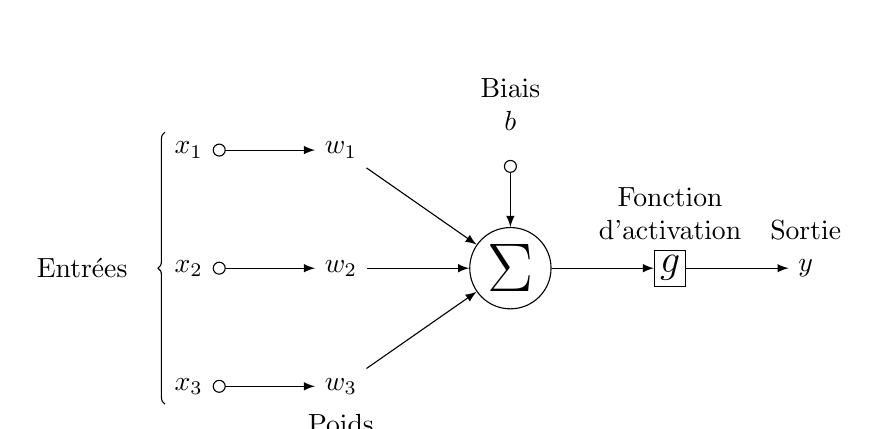
\begin{tikzpicture}[
        init/.style={
          draw,
          circle,
          inner sep=2pt,
          font=\Huge,
          join = by -latex
        },
        squa/.style={
          draw,
          inner sep=2pt,
          font=\Large,
          join = by -latex
        },
        start chain=2,node distance=13mm
        ]
        \node[on chain=2] 
          (x2) {$x_2$};
        \node[on chain=2,join=by o-latex] 
          {$w_2$};
        \node[on chain=2,init] (sigma) 
          {$\displaystyle\Sigma$};
        \node[on chain=2,squa,label=above:{\parbox{2cm}{\centering Fonction \\ d'activation}}]   
          {$g$};
        \node[on chain=2,label=above:Sortie,join=by -latex] 
          {$y$};
        \begin{scope}[start chain=1]
        \node[on chain=1] at (0,1.5cm) 
          (x1) {$x_1$};
        \node[on chain=1,join=by o-latex] 
          (w1) {$w_1$};
        \end{scope}
        
        \begin{scope}[start chain=3]
        \node[on chain=3] at (0,-1.5cm) 
          (x3) {$x_3$};
        \node[on chain=3,label=below:Poids,join=by o-latex] 
          (w3) {$w_3$};
        \end{scope}
        
        \node[label=above:\parbox{2cm}{\centering Biais \\ $b$}] at (sigma|-w1) (b) {};
        
        \draw[-latex] (w1) -- (sigma);
        \draw[-latex] (w3) -- (sigma);
        \draw[o-latex] (b) -- (sigma);
        
        \draw[decorate,decoration={brace,mirror}] (x1.north west) -- node[left=10pt] {Entrées} (x3.south west);
    \end{tikzpicture}
    
    \caption{Schéma d'un neurone artificiel}
\end{figure}{}




\subsubsection{Réseau de neurones}
Les réseaux de neurones artificiels ont été créés en prenant pour inspiration le fonctionnement d'un cerveau, où des enchaînements de neurones émergent des comportements complexes et capables d'apprentissage.
Depuis peu, les réseaux de neurones artificiels connaissent une montée en popularité grâce à des avancées majeures les rendant de plus en plus efficaces, de plus en plus facilement.
\par
Il existe plusieurs architectures de réseaux de neurones artificiels destinés à des usages plus ou moins complexes et spécifiques. Dans notre cas, nous nous cantonneront à l'utilisation de réseaux de neurones à propagation avant (Feedforward Networks), qui sont parmi les architectures de réseaux les plus simples. Ce genre de réseau est constitué d'une couche de neurones en entrée (Input Layer), d'une couche de neurones en sortie (Ouput Layer), et d'un nombre arbitraire de couches intermédiaires (Hidden Layers).
\par
Un réseau de neurones n'est en résumé qu'une fonction à $n$ entrées et $m$ sorties. Pour cela, il est constitué d'un Input Layer et d'un Output Layer contenant respectivement $n$ et $m$ paramètres. Dans le cas d'un réseau Feedforward, les valeurs de sortie des neurones de chaque couche sont calculées à l'aide des valeurs de sortie de la couche précédente, jusqu'à arriver à l'Output Layer. Chaque neurone d'une couche utilise en entrée toutes les sorties de la couche précédente, à l'exception de la première couche où le $i$ème neurone reçoit la $i$ème entrée.
\par


\begin{figure}
    \centering
    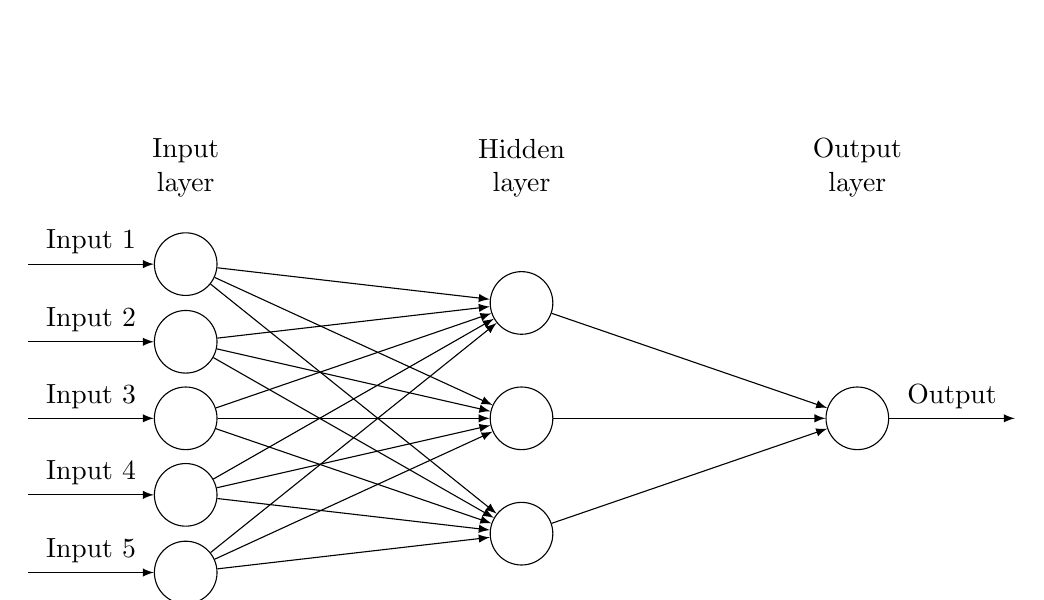
\begin{tikzpicture}[
        plain/.style={
          draw=none,
          fill=none,
          },
        net/.style={
          matrix of nodes,
          nodes={
            draw,
            circle,
            inner sep=8pt
            },
          nodes in empty cells,
          column sep=2cm,
          row sep=-9pt
          },
        >=latex
        ]
        \matrix[net] (mat)
        {
        |[plain]| \parbox{1.3cm}{\centering Input\\layer} & |[plain]| \parbox{1.3cm}{\centering Hidden\\layer} & |[plain]| \parbox{1.3cm}{\centering Output\\layer} \\
        & |[plain]| \\
        |[plain]| & \\
        & |[plain]| \\
          |[plain]| & |[plain]| \\
        & & \\
          |[plain]| & |[plain]| \\
        & |[plain]| \\
          |[plain]| & \\
        & |[plain]| \\    };
        \foreach \ai [count=\mi ]in {2,4,...,10}
          \draw[<-] (mat-\ai-1) -- node[above] {Input \mi} +(-2cm,0);
        \foreach \ai in {2,4,...,10}
        {\foreach \aii in {3,6,9}
          \draw[->] (mat-\ai-1) -- (mat-\aii-2);
        }
        \foreach \ai in {3,6,9}
          \draw[->] (mat-\ai-2) -- (mat-6-3);
        \draw[->] (mat-6-3) -- node[above] {Output} +(2cm,0);
    \end{tikzpicture}
    \caption{Exemple de réseau de neurones à 5 entrées, avec une couche cachée de 3 neurones, et 1 sortie}
\end{figure}{}




\subsection{Apprentissage d'un réseau de neurones}
Comme évoqué précédemment, l'un des intérêts des réseaux de neurones est leur capacité d'apprentissage. Par apprentissage, on désigne la capacité du réseau à se modifier afin d'arriver à produire une valeur attendue quelque soit l'entrée. Dans le cas d'un réseau Feedforward, les valeurs à modifier sont les poids et les biais de chaque neurone.
Plutôt que de modifier radicalement ces valeurs, celles-ci sont modifiées très légèrement, mais sur un nombre important de données. L'objectif est que de ces entraînements résulte un réseau capable de donner une sortie acceptable quelque soit l'entrée qui lui est fournie, même si le réseau n'a jamais été entraîné sur cette entrée précise.
\par
Il est important de bien choisir l'architecture du réseau ainsi que ses hyperparamètres, c'est majoritairement ces choix qui définiront la qualité de l'apprentissage. 

\subsubsection{Architecture}
Dans le cas d'un réseau Feedforward, choisir l'architecture, c'est choisir le nombre d'Hidden Layers et le nombre de neurones de chacun. Plus le nombre d'Hidden Layer est élevé, plus le réseau représentera le problème de manière complexe, ce qui est désirable si le problème est réellement complexe, mais qui peut freiner l'apprentissage et mener à de l'overfitting (sur-ajustement) si le problème est en réalité simple. Le nombre de neurones est lui aussi lié à la complexité du problème, plus un problème est complexe, plus le nombre de neurones devrait être important. Malgré les recherches actives sur le sujet, il n'existe actuellement aucune règle empirique sur le choix du nombre d'Hidden Layer et de neurones. Lorsqu'il est réalisé par un humain ce choix est souvent basé sur l'expérience. Bien que nous ne l'utiliseront pas dans le cadre du projet, une solution efficace à ce problème est l'utilisation d'algorithme génétique appliqué à l'architecture du réseau.

\subsubsection{Hyperparamètres}
On désigne par hyperparamètres toutes les variables qui influent sur l'apprentissage de l'ensemble du réseau. Les plus importants sont généralement le learning rate $\alpha$ et le facteur d'actualisation $\gamma$.
De même que pour l'architecture du réseau il n'existe pas de valeur parfaite pour chaque hyperparamètre, elles dépendront du type de données que l'on souhaite faire apprendre au réseau. Et bien que ce ne soit pas utilisé dans ce projet, il existe des méthodes pour trouver de bonnes valeurs comme le Grid Search, le Random Search, ou encore la plus compliqué Bayesian Optimisation. Bien que très efficaces, il nous a été impossible d'inclure ces méthodes dans le cadre temporel de cette UE.

\subsubsection{Apprentissage}
Les réseaux de neurones sont typiquement entraînés à l'aide de rétropropagations du gradient, qui consistent à donner un couple $(entree, sortie\_attendue)$, et à calculer à l'aide d'une fonction donnée (la fonction de perte) l'erreur entre la sortie attendue et la sortie que le réseau produit. Cette erreur est ensuite propagée de la couche de sortie jusqu'à la couche d'entrée en modifiant à chaque couche les poids de ses neurones pour tenter de minimiser l'erreur.
Si l'architecture du réseau est adaptée au problème et si les hyperparamètres du réseau sont bien choisis, ce dernier devrait aboutir à une configuration de ses poids permettant de donner (en quelque sorte de ``déduire'') la sortie de façon correcte quelque soit l'entrée.
\par


\subsection{Problèmes d'apprentissage}
\subsubsection{Sur-apprentissage}
La façon la plus simple de rater l'apprentissage est de tomber dans un problème de \textbf{sur-apprentissage} (ou sur-interprétation), le réseau est alors trop adapté aux données qui lui on été fournies à l'entraînement, et se montre très peu performant lorsque testé sur des données neuves. Il existe deux façon principale d'arriver à un réseau en sur-apprentissage.

\par
La première est de simplement fournir des données trop peu variées au réseau, qui fonctionnera alors parfaitement sur ces données, mais qui se retrouvera avec des sorties largement incorrectes une fois de nouvelles données fournies. Pour éviter cet écueil, il est pratique courante de mettre de côté un certain nombre de données qui ne seront utilisées que pour les tests, et d'utiliser le reste (la majorité) pour l'entraînement. De cette façon, on peut évaluer le réseau sur des données qui lui sont inconnues.
\par
La deuxième méthode pour tomber dans le sur-apprentissage est de choisir une architecture de réseau trop complexe pour représenter le problème donné. La représentation interne du réseau sera retrouvera trop complexe pour pouvoir interpréter ``simplement'' les données.

\begin{figure}
    \centering
    \includegraphics[width=0.7\textwidth]{images/graph_overfitting.png}
    \caption{Voici un exemple d'overfitting : à partir de points tous à y=0, il est possible de déduire une réalité complexe mais fausse (la fonction sin) (la fonction attendue était f(x)=0).}
\end{figure}{}


\subsubsection{Non convergence}
L'objectif lors de l'entraînement d'un réseau, est de converger vers une disposition des poids où l'erreur sur le noeud de sortie est minimale quelque soit l'entrée. Cependant, il est possible de ne jamais parvenir à approcher une erreur faible.
\par
Une cause possible évidente de ce problème est l'architecture du réseau si cette dernière n'est pas assez complexe pour que le réseau puisse modéliser la solution. Par exemple, une propriété connue des réseaux de neurones est qu'il faut au moins 1 Hidden Layer pour que la sortie ne soit pas linéaire (et 2 Hidden Layers suffisent à modéliser n'importe quelle fonction), ce qui veut dire que la fonction XOR est impossible à faire apprendre à un réseau sans Hidden Layer.
\par
Ce problème peut aussi apparaître si les hyperparamètres sont mal choisis. Si on regarde le cas du facteur d'apprentissage $\alpha$ précédemment présenté, on peut déduire qu'un grand nombre de valeurs possibles mèneront difficilement à une solution : s'il est trop grand, l'ancienne valeur de $Q(s,a)$ sera trop vite écrasée et on perd l'aspect "mémorisation" recherché. S'il est trop petit, l'ancienne valeur de $Q(s,a)$ joue une part trop importante et l'apprentissage ne se fait presque pas. De même pour $\gamma$ dont nombre de valeurs rendent l'apprentissage impossible.
\par
Il est donc extrêmement important de choisir l'architecture et les hyperparamètres du réseau en fonction du problème à traiter sous peine de ne pouvoir jamais aboutir à une solution.


\section{Deep Q-Learning (DQN)}
\subsection{Principe}
Comme évoqué précédemment, le Q-Learning possède des défauts que le Deep Learning semble résoudre. Notre objectif est donc de remplacer le Q-Learning par du Deep Learning, et faire ainsi de l'apprentissage par renforcement sur des réseaux de neurones.
Pour cela, nous remplaçons la Q-Table par un réseau de neurones profond. Le rôle de ce réseau est d'approximer la fonction $Q(s,a)$ : le réseau prend en entrée un état $s$ et donne en sortie les $Q(s,a)$ pour chaque action.

\subsection{Fonctionnement}
Le fonctionnement d'un agent utilisant le Q-Learning ou le DQN pour agir dans son environnement est strictement identique : à chaque état $s$, on choisit une action $a$ à l'aide de notre structure de donnée propre (ou en choisissant une action au hasard, selon la politique en vigueur). L'agent utilisant le Q-Learning choisit la case avec la valeur la plus grande de la ligne $s$ de son tableau, tandis que l'agent DQN fournit son état $s$ en entrée du réseau de neurones, et choisit la sortie ayant la plus grande valeur.
\par
Il n'y a donc aucune difficulté apparente de ce côté, les différences majeures se trouvent à l'apprentissage.
Avec le Q-Learning, ce dernier est relativement simple : c'est un processus itératif où les valeurs de la Q-Table sont peu à peu changées pour converger vers une fonction Q(s,a) (dans ce cas représentée par la table) optimale. 
\par
Cependant l'apprentissage d'un réseau de neurones est bien plus complexe, et on remarque dans la partie précédente que la grande difficulté des réseaux de neurones et de réussir à leur faire apprendre une fonction efficacement. Le nombre de problèmes entravant l'apprentissage est significatif.
\par
Pour régler ces problèmes et tirer plein parti du potentiel du Deep Learning, il est nécessaire de mettre en place certaines optimisations. Nous allons donc tenter d'expliciter les plus élémentaires.

\subsection{Experience Replay}
\subsubsection{Approche simpliste}
Avec le Q-Learning, pour savoir comment changer les valeur de sa table, l'agent utilise simplement la transition $(s,a,r,s')$ obtenu après chaque action effectuée ($s$ correspond à un état, $a$ est l'action effectuée à l'état $s$, $r$ est la récompense obtenue suite à l'action $a$ à l'état $s$, et $s'$ est l'état résultat de l'action).
Bien que simple, cette approche est efficace à résoudre les problèmes pour lesquels le Q-Learning est destiné, la convergence vers une solution étant généralement garantie.
\par
Cette approche est en revanche grandement inefficace lorsque appliquée à des réseaux de neurones. Entraîner des réseaux de neurones sur des données successives rend très difficile les chances d'aboutir à un réseau entraîné pour être optimal en tout état. Les chances d'être constamment dans des minimum locaux ou d'être dans une situation d'overfitting adaptée seulement aux données récentes sont bien trop grandes. Ainsi, l'apprentissage s'en retrouve chaotique, instable et inefficace.

\subsubsection{Principe et fonctionnement}
\par
Une solution possible à ces problèmes est la technique de l'\textbf{Experience Replay}, qui consiste à stocker chaque transition $(s,a,r,s')$ dans un buffer, puis à piocher aléatoirement un nombre arbitraire de transitions, et d'entraîner le réseau sur chacune d'entre elles.
\par
En pratique, on utilisera une file de taille fixe afin que les transitions les plus récentes remplacent les plus vieilles. La taille d'Experience Replay la plus populaire est actuellement $10^6$, mais certains papiers soulignent l'importance de bien choisir cet hyperparamètre qui a un impact important sur l'apprentissage \cite{exp_replay_deeper}.
\par
L'algorithme classique d'apprentissage par renforcement avec Experience Replay est donné plus bas.

\begin{algorithm}
\SetAlgoLined

Initialiser l'Experience Replay $M$\\
\Tq {l'apprentissage n'est pas terminé}
{
Placer l'agent dans un état initial\\
\Tq{l'agent n'est pas dans un état terminal}
{
Sélectionner une action $a$ à effectuer d'après la politique actuelle \\
Appliquer l'action $a$ \\
Observer le nouvel état $s'$ et récupérer la récompense $r$\\
Ajouter la transition $(s,a,r,s')$ à $M$\\
Sélectionner un échantillon aléatoire $B$ dans $M$\\
Faire apprendre au réseau d'après chaque transition de $B$
}
}

\caption{Algorithme classique d'apprentissage utilisant l'Experience Replay}
\end{algorithm}

A chaque ``étape'' ou ``pas'' de l'environnement observé (chaque action effectuée), l'agent choisit une action et l'applique,  mémorise la transition résultante, puis entraîne le réseau sur un échantillon de l'Experience Replay $B$. Cet échantillon est communément appelé \textbf{minibatch}.


\subsubsection{Conséquences}
L'utilisation de l'Experience Replay permet d'enlever tout lien de causalité entre chaque action et de permettre au réseau un apprentissage bien plus général du problème. Cela permet aussi de ne pas apprendre des transitions dépendant exclusivement de la politique actuelle de l'agent, on peut par exemple trouver dans l'Experience Replay des transitions effectuées lorsque l'agent avait son hyperparamètre $\epsilon$ égal à 1 alors que sa valeur actuelle est bien plus basse. On en déduit par la même occasion que grâce à l'Experience Replay, le réseau est susceptible d'apprendre plusieurs fois une même transition (à des instants différents) \cite{atari_drl}.
\par
Toutes ces propriétés de l'Experience Replay permettent de contourner les problèmes précédemment évoqués, et bien que cette méthode soit globalement assez efficace pour permettre un bon apprentissage dans les problèmes que nous traitons, l'Experience Replay implique un défaut majeur : l'apprentissage des transitions nouvellement effectuées (potentiellement très cruciales à l'apprentissage) ne se fait pas instantanément, il faut avoir la ``chance'' que l'agent tombe dessus lors de la pioche aléatoire de transitions. Bien que des améliorations du principe ont été créées (Prioritized Experience Replay), à la date de création de ce rapport il semble qu'aucune alternative majeure à l'Experience Replay n'existe.

\subsection{Standardisation des entrées}
Un réseau de neurones accepte en entrée un certain nombre de réels. Les réels peuvent être de n'importe quelle valeur, en théorie cela ne devrait pas poser de problème au réseau : en cas de problème et avec un nombre suffisant d'Hidden Layers, le réseau pourra ``redimensionner'' ces valeurs de façon à contrer la disproportion de grandeurs.
\par
Par exemple, il est possible qu'un des réels fournis en entrée d'importance moindre soit significativement plus grand qu'un autre réel dont l'importance est majeure : mathématiquement, ce n'est pas ce que l'on désire. On sait que le réseau pourra annuler et renverser ce déséquilibrage au fil de l'apprentissage grâce à ses Hidden Layer.
\par
Toutefois, il est très commun de malgré tout normaliser les entrées, que ce soit pour simplement tous les faire tenir dans un intervalle plus réduit (typiquement $[0;1]$ ou $[-1;1]$ ) en redimensionnant toutes les entrées, ou pour ramener toutes les entrées à des ``importances'' identiques en appliquant un redimensionnement adapté à chaque entrée.
\par
Appliquer ce redimensionnement au préalable (en pré-processing) permet d'éviter de complexifier inutilement l'apprentissage du réseau. De plus, les poids du réseau sont initialisés par des valeurs arbitraires, généralement adaptées à des valeurs d'entrée faibles, redimensionner les entrées du réseau permet d'éviter d'adapter ces valeurs.
\par
Ainsi en pratique on normalisera les entrées dès que c'est possible afin de faciliter et accélérer l'apprentissage \cite{ai_faq}.


\subsection{Dropout}
Bien qu'elle soit moins essentielle en reinforcement learning où l'on peut obtenir un nombre quasi infini d'informations pour entraîner le réseau de neurones, la méthode de \textbf{Dropout} (ou ``Abandon'') est un moyen très simple et efficace de réduire le surajustement du réseau.
\par
Son principe est extrêmement simple : lors de l'entraînement, chaque neurone a une chance $p$ d'être ``désactivé'' sa valeur de sortie est alors 0 (il n'a aucune influence sur le réseau). En revanche lors de phases de test (lorsqu'un utilise le réseau), tous les neurones se comportent normalement.

\begin{figure}
    \centering
    \includegraphics[width=1\textwidth]{images/dropout.png}
    \caption{\textbf{A gauche} (a) : réseaux neuronal standard avec 2 couches cachées. \textbf{A droite} (b) : le même réseau après application du Dropout. Les neurones avec une croix ont été désactivé (drop).
    \\\textit{Schéma tiré du papier original sur le Dropout} \cite{dropout}}
\end{figure}

\par
Il est assez intuitif de comprendre le fonctionnement de cette technique : le réseau évitera de faire de mauvaises ``conjecture'' parce que par coïncidence des neurones s'activent en même temps. Au fil de l'entraînement, on n'entraîne que certaines parties du réseau seulement sur une certaine partie des données (les neurones de la couche d'entrée sont eux aussi susceptibles d'être désactivés).
\par
A la fin de l'entraînement, les chances du réseau d'effectuer de mauvaises ``conjectures'' suites à des coïncidences dans ses données et dans son entraînement seront grandement réduites, et le réseau s'en retrouve en conséquence bien plus efficace.
\par
En pratique, la valeur de $p$ la plus utilisée est $0.5$, qui d'après les études menées sur le sujet, correspond à la grande majorité des situations \cite{dropout}. 

\chapter{Conception}


\section{Planification}

La planification du projet est présentée en détails plus bas. Concernant la gestion interne des taches et de leur avancement, nous utilisons Trello comme requis par l'enseignant responsable de l'UE, en voici le lien d'invitation : \\ \url{https://trello.com/invite/b/HUauMOnv/41ec23e7edb8b51517df475551b7f823/ia-reinforcement-learning}


\begin{center}
\begin{tabularx}{\linewidth}{|p{1cm}|X|p{2.1cm}|p{1cm}|}
    \hline
    ID & Tâche & Antécédents & Durée \\
    \hline
    \hline
    A & Étude de recherche de trésor 1D avec Q-Table & / & 2h \\
    \hline
    B & Programmation de l'IA recherche de trésor 2D avec Q-Table& A & 2h \\
    \hline
    C & Étude du Deep Reinforcement Learning & B & 6h \\
    \hline
    D & Développement d’un environnement générique pour la recherche de trésor & A & 2h \\
    \hline
    E & Développement d’un agent DQN & C & 4h \\
    \hline
    F & Création d’une interface basique & / & 1h \\
    \hline
    G & Création d’une interface avancée & F & 4h \\
    \hline
    H & Développement du système de sauvegarde/chargement d’IA & E & 4h \\
    \hline
    I & Développement du mode ``joueur'' & / & 2h \\
    \hline
    J & Développement d’un agent double DQN & E & 6h \\
    \hline
    K & Développement des tests de l’IA & E & 4h \\
    \hline
    L & Développement d’un agent Q-learning & A & 2h \\
    \hline
    M & Développement du visionnage de l’IA en temps réel & F,L & 2h \\
    \hline
    N & Développement d’agents  RL bonus (si il nous reste du temps après avoir terminé toutes les tâches ci-dessus) & D, G, H, I, J, K, M & 8h \\
    \hline
\end{tabularx}
\end{center}

\begin{figure}
\centering
\includegraphics[width=1\textwidth]{pert.png}
\caption{Diagramme de PERT du projet}
\end{figure}

\begin{figure}
\centering
\includegraphics[width=1\textwidth]{gantt.png}
\caption{Diagramme de Gantt original du projet}
\end{figure}

\begin{figure}
\centering
\includegraphics[width=1\textwidth]{gantt_2p.png}
\caption{Diagramme de Gantt adapté à deux personnes}
\end{figure}

L'étape de planification est probablement l'étape du projet la plus complexe à effectuer correctement, c'est donc sans surprise que la planification originalement prévue n'a pas du tout correspondu à la réalité.
\par
La durée estimée de la plupart des tâches était totalement incorrecte, en majorité parce que nous sous-estimions la durée des tâches à effectuer. Le diagramme était pensé pour correspondre au nombre d'heures allouées à l'UE, mais il est en réalité totalement impensable de réussir à terminer ce projet en ne travaillant dessus que 4 heures par semaine.
\par
Le premier objectif du projet fut accompli très rapidement, plus tôt que ce que le diagramme de Gantt prévoyait. Mais le second objectif se révéla être bien plus complexe que prévu, et demanda un grand nombre d'heures de test, de recherche et d'entraînement.
\par
Vous trouverez néanmoins dans cette partie l'ensemble des diagrammes planifiant le déroulement du projet.

\FloatBarrier

\section{Réalisation de la première partie}

La première partie du projet est la réalisation d'un agent capable de jouer (et résoudre, si possible) à la recherche de trésor.

\subsection{Résumé du déroulement}
Bien que la tâche soit relativement simple, au moment où nous commencions le projet, nous ne disposions d'aucune expérience préalable dans le domaine de l'apprentissage par renforcement. Il nous a donc dû fallu nous instruire sur le sujet à l'aide de différentes ressources : cours, articles et exemples.
\par
Notre professeur référent Mme Li nous a redirigé vers son cours sur l'apprentissage par renforcement qu'elle dispense en master, et qui contient une introduction à l'intelligence artificielle, dont l'apprentissage par renforcement à l'aide de Q-Learning \cite{li_rl}. Nous avons aussi consulté différents articles introductifs à l'apprentissage par renforcement, et nous sommes appuyé d'un livre introductif sur le sujet pour en savoir plus sur certains points \cite{rl_an_intro}. Enfin, afin d'observer comment sont implémentées ces connaissances en pratique, nous avons cherché différentes implémentations de Q-Learning que nous avons copié, exécuté, et modifié afin de tenter d'en comprendre le fonctionnement et les structures utilisées \cite{morvanzhou}.
\par
Une fois cette phase de recherche effectuée, nous avons commencé à réimplémenter par nous même le Q-Learning sur la recherche de trésor en 1D. Le principe fut assez vite compris, et la seule difficulté rencontrée était l'utilisation de librairie externe pour manipuler plus rapidement la Q-Table. Suite à cet accomplissement, nous avons reporté notre avancement à notre professeur référent qui nous a proposé d'essayer d'appliquer l'algorithme sur une recherche de trésor en 2D. Cette tâche fut elle aussi assez rapidement effectuée et ne posa pas de problème particulier. Nous nous décidâmes donc à commencer la deuxième partie du projet.

\subsection{Détails de la phase d'implémentation}
Une de premières choses que nous avons fait était de copier un programme déjà existant solvant la recherche de trésor en 1D, et d'en comprendre le fonctionnement. Avant même de tenter de le modifier, nous nous sommes heurté à un problème de compréhension sur le fonctionnement de la Q-Table. Nous avons donc consulté les différentes ressources citées precedemment au fil de notre tentative de compréhension du code afin de comprendre ce qui s'y déroulait exactement.
\par
Une fois le principe de Q-Table compris, nous nous sommes attelé à réécrire le programme de façon plus concise à partir de ce que nous avions compris (l'environnement étant extrêmement simple, la majorité du code n'est que l'agent). La seule partie d'ombre sur le programme était l'affectation tirée de l'équation de Bellman, que nous avions du mal à comprendre intuitivement.
\par
Nous avons ensuite enchaîné sur l'application de notre agent sur un environnement en 2D, et par la même occasion le code fut entièrement réécrit afin de rendre le tout plus propre et compréhensible : le programme en 1D étant très fouillis et confus en raison des essais et modifications pour mieux comprendre son fonctionnement. Cette réécriture fut aussi l'occasion de tester l'orienté objet en Python, qui nous sera utile pour faire des programmes plus conséquents et mieux structurés.
\par
La recherche de trésor en 2D ne posa pas de problème particuliers et ce fut l'occasion de vérifier que nous comprenions bien le fonctionnement d'un agent utilisant le Q-Learning. Seul un point restait quelque peu abstrait : les valeurs des hyperparamètres. Jusqu'ici, nous n'avions pas eu besoin d'y toucher, leur valeurs étaient fixées à $\alpha=0.1$ et $\gamma=0.9$. Bien que nous connaissions leur ``sens'' théorique, notre faible expérience nous empêchait de bien concevoir leur conséquence sur l'apprentissage.

\section{Réalisation de la seconde partie}
La seconde partie du projet est celle ayant posé le plus de problèmes et nous ayant pris le plus de temps. Elle consiste à utiliser le Deep Q-Learning afin de développer un agent capable de jouer à Pac-Man.

\subsection{Choix de l'environnement}
Il est important de noter que OpenAI Gym propose deux versions de chaque jeu Atari où l'état observé par l'agent diffère : dans la première version (nommée \textit{nomjeu-v0}) l'agent observe l'écran du jeu, tandis que dans la deuxième version l'agent observe la RAM du jeu (les jeux Atari 2600 possèdent 128 octets de RAM).
\par
Initialement, nous avions envisagé d'utiliser l'environnement fournissant l'image, puisque cette approche semblait plus ludique et intuitive, toutefois elle requiert quelques connaissances de plus. Nous avons finalement décidé de d'abord ``résoudre'' l'environnement RAM, et si nous avions du temps restant, de résoudre l'environnement avec image.

\subsection{Prémices de la création de l'agent DQN}
L'environnement n'étant pas à notre charge, nous avons directement entamé des recherches pour comprendre le principe du Deep Q-Learning. Bien que son résumé soit simple : ``un réseau de neurone approxime la fonction Q'', cette nouvelle approche apporte son lot de questions et de nouvelles connaissances.
\par
Il nous a d'abord fallu nous mettre à niveau au sujet des réseaux de neurones que nous n'avions alors pas encore abordé lors de notre cursus universitaire \cite{dl_mit, 3b1b_nn, colah}. Dans le même temps, nous tentions de comprendre comment fonctionnait le Deep Q-Learning. Une des difficultés est de réussir à comprendre quels éléments sont des composants essentiels, et quels composants sont des améliorations créées pour rendre le DQN plus efficace. Il est en effet très commun de trouver des implémentations d'agents Double DQN dans des tutoriels, mais commencer par essayer de comprendre une version améliorée du principe rend la tâche plus complexe. Nous avons malgré tout réussi à saisir le fonctionnement du Deep Q-Learning grâce à quelques cours, articles et implémentations \cite{stanford_drl, atari_drl, keon}.

\subsection{Implémentation et premiers tests}
Comme pour la première partie, programmer l'agent fut assez rapide. L'essentiel de la difficulté se trouvant dans le principe, le code n'est pas spécialement long. Une fois implémenté, et pour en tester le bon fonctionnement, nous avons décidé de tester l'agent sur l'environnement de recherche de trésor 2D avec obstacles.
\par
Nous avons été confrontés à notre premier problème de définition de structure du réseau : combien de couches le réseau a-t-il besoin ? Combien de neurones chaque couche doit-elle avoir ?
Nous avons dans un premier temps effectués quelques essais à l'aveugle, avec pour seule connaissance utile que deux couches cachées suffisent à représenter n'importe quelle fonction. Nous supposions que par exemple, dans un environnement à 100 états possibles, un réseau de deux couches cachées de 10 neurones pourrait fonctionner. Mais après quelques essais aléatoires infructueux nous avons décidé de rechercher comment choisir l'architecture d'un réseau selon le problème.
\par
A notre grande surprise, nous avons trouvé qu'il n'existait aucune méthode fiable pour choisir ces paramètres du réseau, c'est majoritairement à l'expérience que la plupart des gens estiment grossièrement l'architecture que le problème requiert. Pour obtenir des architectures optimales il est nécessaire d'utiliser des méthodes capables de faire évoluer l'architecture, il nous est cependant impossible d'en arriver à utiliser de telles méthodes.
\par
Après d'autres essais infructueux, nous commencions à penser que le problème venait sûrement du type d'environnement. En effet, la recherche de trésor est particulièrement basé sur la mémorisation, et surtout sa seule récompense est obtenue en arrivant sur la dernière case. Ce qui veut dire que dans un premier temps, l'agent doit trouver au hasard le trésor, ce qui peut prendre un temps extrêmement long (et qui augmente exponentiellement avec la taille de l'espace de jeu). Puis l'agent doit apprendre le chemin qui remonte jusqu'au trésor à partir de cette seule information. 
\par
De plus, et bien que ce n'est que plus tard que nous l'avons compris avec les recherches pour la partie ``principe des algorithmes utilisés'', l'Experience Replay rend l'apprentissage encore plus complexe. En effet, pour que le réseau apprenne à aller jusqu'à la case d'arrivée, il faut d'abord que la transition de récompense non nulle soit présente dans un des minibatch, selon la taille de l'Experience Replay, du minibatch, et de l'environnement, tomber dessus peut s'avérer très rare.
\par
La recherche de trésor telle que nous l'avons implémenté est donc bien un très mauvais exercice pour les agents DQN, le point majeur à changer dans cet environnement est la fonction de récompense qui donne trop peu d'information sur la performance de l'agent (seulement gagné ou perdu).

\subsection{Première application à Pac-Man}
Suite à nos échecs sur la Recherche de trésor, nous avons décidé de tester l'agent DQN sur Pac-Man. Encore une fois, nos essais se sont tous soldés par des échecs : au terme de l'apprentissage, Pac-Man se retrouvait très souvent bloqué dans des coins sans jamais bouger. Nous ne constations aucune tentative de collecter le maximum de points.
\par
Très vite, nous avons repéré un premier problème : le jeu ne possède pas de récompense négative, la fonction de récompense correspond simplement au score gagné à la frame jouée. OpenAI Gym donnant avec ses environnements l'accès à quelques variables supplémentaires, nous avons pu rajouter une récompense négative dans le cas où le Pac-Man perd une vie (ce qui arrive environ une demi seconde après qu'il ait tué un fantôme).
\par
Cette modification n'a malheureusement pas suffit à améliorer le comportement de l'agent. Notons qu'à ce moment, nous avions déjà implémenté un système de décroissance de la valeur d'$\epsilon$, qui permet de transitionner de choix d'action aléatoire vers un choix plus "raisonné". Mais peu importe la vitesse de décroissance choisie, l'agent n'arrivait pas à un résultat convenable. Ici encore nous avons tenté plusieurs approches d'architecture, mais ici aussi nos essais se sont tous soldés par des échecs.
\par
Il faut aussi noter qu'à cause du système d'apprentissage par minibatch à chaque étape de jeu, la vitesse de jeu est extrêmement lente, et il faut laisser tourner le jeu de nombreuses heures avant d'être sûr de la qualité de l'agent.

\subsection{Application à Cartpole}
Incapable de faire fonctionner l'agent sur Pac-Man, et surtout incapable de trouver un exemple d'architecture ayant déjà résolu ce problème (en apprentissage par renforcement, les jeux Atari 2600 sont relativement communs, mais c'est en général la version où l'agent lit l'écran qui est utilisée), nous décidâmes de tester notre agent sur un environnement plus commun et déjà résolu.
\par
Cartpole est un environnement très simple : dans un environnement en deux dimensions, vu de côté et avec la gravité vers le bas, il faut maintenir un baton à la verticale en déplaçant le chariot le soutenant vers la gauche ou vers la droite.

\begin{figure}
    \centering
    \includegraphics[width=1.0\textwidth]{images/cartpole.png}
    \caption{Représentation graphique de l'environnement CartPole-v1}
    \label{fig:my_label}
\end{figure}

L'environnement observé fournit quatre réels pour décrire son état : la position du chariot, la vitesse du chariot, la rotation du baton et la vitesse de rotation du baton. Les deux actions possibles sont d'accélérer le chariot vers la gauche ou vers la droite. L'objectif est de maintenir le baton à la verticale, l'agent obtient 1 de récompense pour chaque étape de jeu. Le jeu est de durée fixée et ne peut durer plus de 200 étapes. Le jeu est perdu si l'angle du baton par rapport à la verticale est supérieur à 15 degrés.
\par
Cet environnement est extrêmement pratique pour les tests, il est bien connu et on connaît des architectures et hyperparamètres qui fonctionnent. Nous avons donc cherché une solution existante \cite{gsurma_cartpole} et copié ses hyperparamètres et l'architecture de son réseau de neurones.
\par
L'apprentissage a marché sans aucun problème, avec quelques ajustement, nous avons même réussi à obtenir un réseau atteignant un score maximal au bout de 100 épisodes (ce qui arrive très rapidement). Ce test avec CartPole nous a permit de vérifier le bon fonctionnement des algorithmes utilisés par notre agent.
\par
Nous tirons comme conclusion de cette essai que le problème jusqu'ici ne vient pas de notre implémentation d'agent DQN, qui fonctionne parfaitement, mais de nos choix d'hyperparamètres, et de notre architecture de réseau.

\subsection{Application à Breakout}
Pac-Man est un jeu complexe : l'agent doit collecter différents bonus disséminés dans un labyrinthe tout en évitant les ennemis qui le poursuivent. De plus, l'environnement fournit à l'agent toute la RAM de l'Atari 2600 qui contient 128 entiers compris entre 0 et 255 qui devront permettre à l'agent de déduire quelle action il devra effectuer.
\par
Plutôt que de commencer par Pac-Man (duquel on ne connait pas l'architecture optimale, ni les hyperparamètres optimaux), il serait peut-être bénéfiques de réussir à faire résoudre un environnement Atari plus simple à notre agent. Lors de nos recherches nous avons trouvé un exemple de résolution de Breakout ainsi et surtout qu'un papier détaillant la résolution de jeux Atari 2600 en utilisant leur RAM \cite{breakout_tkgw, learn_atari_ram}.
\par
C'est cette dernière ressource qui a joué un rôle capitale dans notre résolution d'environnement Atari. On y trouve en effet de nombreuses améliorations possibles afin d'augmenter l'efficacité de l'agent. L'application de seulement quelques unes de ces dernières permet d'atteindre des performances tout à fait respectables, capables de faire des scores raisonnables sur Breakout.
\par
Nous avons utilisé les valeurs donné à la fin du papier, ainsi que l'architecture ``small ram'' (deux couches cachées de 128 neurones). Ainsi que les hyperparamètres fournis (la majorité d'entre eux proviens d'un autre papier fondateur sur l'application du DQN aux environnements Atari \cite{atari_drl}. Après environ 4 heures d'entraînement, l'agent dépassait régulièrement un score de 20 et continuait de s'améliorer. Les améliorations utilisées sont la normalisation ainsi que le frame skip (définit à 8).
\par
Le Breakout n'étant pas notre objectif, c'est vers Pac-Man que nous avons redirigé nos efforts avec ces nouvelles connaissances.


\subsection{Application à Pac-Man}
\subsubsection{Résumé des améliorations}
Deux de nos problèmes majeurs avec Pac-Man étaient la vitesse de jeu, très lente et qui empêche à l'agent de recueillir un nombre conséquent de situations par le temps qu'il prend à s'entraîner, ainsi que l'impression que le réseau n'arrive pas à apprendre à partir des données fournies.
\par
Le premier problème est réglé par le principe de ``frame skip'', qui consiste simplement à ne fournir à l'agent qu'un instantanné de la RAM sur $n$. Le jeu tourne originalement à 60 images par secondes, à chaque étape l'agent avance d'une image, après 60 étapes il complète une seconde de jeu. Si on prend un frame skip $n=3$, l'agent ne voit qu'une image sur trois, le jeu est pour lui en 20 images par secondes. Cette approche permet d'augmenter drastiquement la vitesse de jeu sans nécessairement y perdre en précision : le jeu est créé pour être joué par un humain ne disposant pas de la capacité d'analyser le jeu 60 fois par secondes. Le seul problème possible peut se présenter si le joueur doit bien ``timer'' ses actions, ce qui n'est pas le cas dans Pac-Man.
\par
Le second problème est réglé par l'utilisation de la normalisation. Cette dernière est très simple : on possède en entrée une liste de 128 octets représentés par des entiers entre 0 et 255, pour les normaliser ont divise simplement l'ensemble de ces entiers par 255. Grâce à cette normalisation, nous nous retrouvons avec une liste de réels compris entre 0 et 1, facilitant ainsi l'apprentissage du réseau de neurones.

\subsubsection{Hyperparamètres et architecture}

Nous réutiliseront les paramètres "classiques" des jeux Atari 2600.

\begin{itemize}
\item learning rate ($\alpha$) = 0.0002
\item discount factor ($\gamma$) = 0.95
\item memory size = $10^6$
\item initial epsilon ($\epsilon$) = 1.0
\item minimal epsilon = 0.05
\item epsilon decay  = 0.997
\item frame skip = 8
\end{itemize}

Notons que $\epsilon$ n'est multiplié par epsilon decay que lorsqu'un épisode est terminé, et non à chaque image de jeu. 
\par
L'architecture de réseau utilisé est calquée sur celle du Breakout : deux couches cachées de 256 neurones chacune (contre 128 pour le breakout, ce choix a été effectué avec l'espoir d'adapter le réseau au nombre d'informations à retenir et prendre en compte dans Pac-Man). La fonction d'activation de ces deux couches est la fonction ReLU, la dernière couche utilise la fonction d'activation identité (ce qui revient au même que n'appliquer aucune fonction).


\subsubsection{Entraînement et analyse des résultats}
Après environ 1000 épisodes d'entraînement, l'agent DQN arrive à dépasser régulièrement un score de 1300. Après 2500 épisodes, nous avons réussi à atteindre un score maximal de 3970.
\par
Nos attentes dans le comportement d'un agent entraîné était que ce dernier apprenne à éviter les fantômes, afin de permettre de survivre le plus longtemps dans le labyrinthe et ainsi augmenter ses chances de compléter le labyrinthe. Cependant, l'agent a trouvé une autre approche bien plus simple et moins subtile : il commence chaque partie par se diriger vers une des quatre super Pac-Gommes, qui permettent à Pac-Man d'être invincible et de manger les fantômes. Il explore ensuite relativement normalement (bien que son exploration soit loin d'être parfaite), en privilégiant l'obtention de super Pac-Gommes. Cette technique, bien que relativement ``bête'' et très éloignée des attentes de techniques d'évitements que nous avions en tête, augmente énormément les chances de faire un score important.




\chapter{Explications du code}

\section{Dépendances et fonctionnements des librairies externes}

\subsection{OpenAI Gym}

OpenAI Gym est une librairie fournissant des dizaines d'environnements destinés à l'apprentissage par renforcement. On y trouve des environnements basé sur la robotique, de simples algorithmes à résoudre, ou encore des jeux Atari 2600. Parmi ces derniers on retrouve Ms. Pac-Man, sur lequel la majorité de notre projet porte.

\subsubsection{Fonctionnement basique}
Le fonctionnement de Gym est globalement très simple, le plus important est sa classe Env, qui contient 3 fonctions principales :
\begin{verbatim}
step(action) -> state, reward, done, info
render()
reset() -> reset
\end{verbatim}
``step'' permet de faire avancer l'environnement d'une étape en appliquant l'action passée en paramètre, il renvoie l'état résultant, la récompense associée, si l'environnement est dans un état terminal, et des informations supplémentaires spécifiques à chaque jeu.
\par
``render'' lancer l'affichage du jeu, soit sous forme textuelle, soit dans une fenêtre séparée selon le jeu. Il est possible de passer en argument un type d'affichage spécifique pour l'enregistrement vidéo par exemple, mais cette fonction ne sera pas utilisée dans le projet.
\par
``reset'' remet simplement l'environnement à zéro et renvoie le nouvel état.
\par
Pour créer un environnement donné, il suffit d'appeler
\begin{verbatim}
import gym

mon_env = gym.make("nom_environnement")
\end{verbatim}
Ici on initialise puis stocke l'environnement nommé ``nom\_environnement'' dans la variable ``mon\_env''.

\subsubsection{Création d'environnement personnalisé}
Afin de rendre les choses plus simples lors de la programmation du logiciel principal, nous avons jugé intéressant de pouvoir directement créer l'environnement de recherche de trésor de façon identique aux reste des environnement.
\begin{verbatim}
gym.make("tresor2d-v0")
\end{verbatim}
Gym permet d'ajouter ses propres librairies, nous avons ainsi porté l'environnement de recherche de trésor en deux dimensions précédemment créé afin qu'il respecte l'interface de Gym \cite{gym_custom_env}.
\par
L'environnement contient ainsi les trois fonctions précédemment citées. Son fonctionnement est simple : il stocke dans un tableau en deux dimensions la topologie du terrain (le type de chaque case : sol, mur, trésor), et dans une variable la position (x,y) du joueur. L'état du jeu correspond à la position du joueur convertie en entier à l'aide de la formule
\[etat=x + y . width\]
où $(x,y)$ la position du joueur et $width$ la largeur du terrain.
\par
L'installation de l'environnement personnalisé se fait par pip, ce qui limite la portabilité du programme. Nous n'avons cependant pas trouvé d'alternative à cette approche.


\subsection{Keras}
Keras offre différentes fonctionnalités pour permettre une utilisation aisée de l'apprentissage profond.

\subsubsection{Création d'un réseau de neurones basique}
Nous n'utiliserons dans notre projet que des réseaux de neurones feedforward. Ces derniers se font très simplement à l'aide de Keras, voici un script python utilisant presque toutes les fonctionnalités de Keras que l'on peut retrouver dans notre projet.

\begin{lstlisting}[language=Python,breaklines=true, caption=Exemple d'utilisation de Keras]
from keras.models import Sequential
from keras.layers import Dense
from keras.models import load_model

#Créer un modèle de couches de neurones séquentiel. Les couches se suivent les unes les autres linéairement
model = Sequential()

#Créer des couches afin d'aboutir à un réseau à 100 entrées,avec deux couches cachées contenant respectivement 8 neurones à activation ReLU et 10 neurones a activation sigmoide, et 2 neurones de sortie à activation linéaire
model.add(Dense(units=8, activation='relu', input_dim=100))
model.add(Dense(units=10, activation='sigmoid'))
model.add(Dense(units=2, activation='linear'))

#Compiler le modèle précedemment défini en utilisant la fonction de perte  Mean Squared Error (Erreur quadratique moyenne) et l'optimizer Adam
model.compile(loss='mse', optimizer='adam')

#Entraîner le reseaux sur un échantillon de données d'entrée x_batch associées à l'échantillon de sorties attendues y_batch
model.train_on_batch(x_batch, y_batch)

#Calcule ce que renvoient les noeuds de sortie du réseau
result = model.predict(x_test)

#Sauvegarde le modèle dans un fichier
model.save("fichier1.h5")

#Charger un modèle depuis un fichier
model2 = load_model("fichier2.h5)

\end{lstlisting}

\subsection{NumPy}
NumPy est une librairie à but ``scientifique'', elle propose des opérations très efficaces sur des tableaux à N dimensions, et possède un grand nombre d'opérations mathématiques de base sur ces derniers.
\par
Dans le cadre de notre projet, NumPy est utilisé principalement pour l'implémentation du Q-Learning et plus précisément la manipulation de la Q-Table. Voici pour exemples quelques unes des utilisations majeures de NumPy dans notre projet :

\begin{lstlisting}[language=Python, breaklines=true, caption=Exemples d'utilisations de NumPy]
import numpy as np


#Exemple d'utilisation de NumPy pour créer la Q-Table initialisée par des 0.
def _build_table(self):
    return np.zeros([self.state_count, self.action_count])

#Utilisation de NumPy pour récupérer aisément la valeur maximale d'une ligne donnée
q_target = reward + self.discount_factor * np.max(self.qtable[new_state])

#Récupérer la meilleure action sur un état, c'est-à-dire récupérer l'indice de la case de valeur la plus importante
best_action = np.argmax(self.qtable[state])
\end{lstlisting}


\section{Structure du projet}

\begin{figure}
    \centering
    \begin{forest}
      for tree={
        font=\ttfamily,
        grow'=0,
        child anchor=west,
        parent anchor=south,
        anchor=west,
        calign=first,
        edge path={
          \noexpand\path [draw, \forestoption{edge}]
          (!u.south west) +(7.5pt,0) |- node[fill,inner sep=1.25pt] {} (.child anchor)\forestoption{edge label};
        },
        before typesetting nodes={
          if n=1
            {insert before={[,phantom]}}
            {}
        },
        fit=band,
        before computing xy={l=15pt},
      }
    [
      [agents]
      [envs
        [gym-tresor2d
            [gym\_tresor2d
                [envs]
            ]
        ]
      ]
      [misc]
      [saves]
    ]
    \end{forest}
    \caption{Arborescence du projet}
\end{figure}{}


Le projet n'est pas d'envergure conséquente et il est simple de le diviser en quelques parties distinctes au rôle défini.
\par
Notons que quelques classe décrites par la suite contiennent des fonctions privées (précédées d'un \_) qui ne seront pas forcément listée. L'ensemble du code est commenté, nous encourageons donc à aller y jeter un oeil dans le cas où vous souhaiteriez plus de détails sur l'implémentation.

\subsection{Dossier ``agents''}
Le dossier agents contient les différents agents du projet. Actuellement, le projet supporte deux types d'agents : l'agent utilisant le Q-Learning, et l'agent utilisant le DQN, respectivement \textit{qlearning\_agent.py} et \textit{dqn\_agent.py}.
\par
\textit{qlearning\_agent.py} contient une unique classe \textbf{QLearningAgent} disposant de fonctions de base d'un agent : \textit{fit} (entraînement), \textit{act} (agir), \textit{save} (sauvegarder), \textit{load} (charger) ainsi qu'une fonction \textit{get\_written\_summary} permettant d'obtenir un bref résumé écrit de l'état de l'agent. 
\par
De même \textit{dqn\_agent.py} contient une unique classe \textbf{DQNAgent} disposant de fonctions des mêmes fonctions de base que QLearningAgent (aux arguments cependant différents selon les fonctions), ainsi que de quelques autres uniques au Deep Q-Learning, comme par exemple \textit{memorize} ou \textit{replay}, liées à l'experience replay.
\par
Ces agents fonctionnent indépendamment du reste du projet et peuvent être utilisés facilement. C'est majoritairement eux qui vont faire l'interface avec les librairies citées précédemment.

\subsection{Dossier ``envs''}
C'est dans ce dossier que se trouve l'environnement de recherche de trésor en deux dimensions. La disposition étrange des dossiers n'est que le résultat des prérequis à son installation par pip, et n'est donc pas un choix délibéré de notre part.
\par
Le seul fichier python contenant réellement du code est \textit{tresor\_env.py}, situé quelques sous-dossiers plus bas. Ce dernier contient l'intégralité du code simulant l'environnement.
\par
Pour la classe \textbf{Tresor2dEnv}, nous avons dû nous plier à l'interface de classe ``Env'' existant dans la librairie Gym. Afin d'implémenter correctement une classe environnement, il faut hériter de la classe ``Env'' et override les fonctions \textit{step}, \textit{reset} et \textit{render}. Comme expliqué plus tôt dans ce rapport, \textit{step} est chargé de faire avancer le jeu d'une étape en prenant une action en argument, \textit{reset} remet l'environnement à son état initial, et \textit{render} affiche graphiquement l'état du jeu.
\par
Pour ce jeu, nous avons simplement stocké l'état du labyrinthe dans un tableau en deux dimension où chaque cellule correspond au terrain de la case, et appliqué un simple test de collision lors des déplacements de la fonction \textit{step}.
\par
Concernant la génération du terrain, rien de compliqué n'a été utilisé, trois types de terrains sont possibles : \textit{empty}, \textit{random} et \textit{zigzag}. Le premier est un simple terrain vide avec le trésor à son extremité, le second contient des obstacles aléatoirement placés en créant un chemin permettant d'arriver à coup sûr au trésor, et le dernier génère un labyrinthe où le chemin à emprunter ``zigzague''.
\par
Il est possible de choisir le type de génération ainsi que la taille du terrain lors de l'appel de la fonction \textit{make} de Gym. Voici un exemple où l'on crée un environnement de recherche de trésor de taille 6x6 et utilisant la génération ``zigzag''.

\begin{lstlisting}[language=Python,breaklines=true, caption=Initialisation d'un environnement tresor-2d]

import gym
import gym_tresor2d
e = gym.make("tresor2d-v0", width=6, height=6, generation_type="zigzag")

\end{lstlisting}


\subsection{Dossier ``misc''}
Le dossier misc (pour ``miscellaneous''), contient différents scripts aux utilités variées. Le projet n'étant pas assez gros pour séparer ces scripts dans plusieurs dossiers sans qu'ils ne se trouvent seuls dans leurs dossiers respectifs, nous avons décidé de rassembler ici tout ce qui ne rentrait pas dans les autres catégories.
\par
On y retrouve ``console\_helper.py'', qui permet de rendre générique l'entrée par l'utilisateur d'une suite de valeurs, ce qui est extremement pratique pour le script principal.
\par
Le fichier ``gameinfo.py`` permet de récupérer facilement les environnements du projet et les informations qui leur sont associés.
\par
Enfin, le fichier ``pacman\_tools.py'' contient les fonction de pré-traitement de l'état du jeu, ainsi que les fonctions permettant de comptabiliser les morts dans la récompense fournie à l'agent.

\subsection{Dossier ``saves''}
Il n'y a pas grand chose à dire sur ce dossier, ci ce n'est que c'est dans celui-ci que seront sauvegardés les données des agents entraînés.


\section{Fonctionnement du projet}

\subsection{Script principal}
Le script principal du projet est ``launcher\_text.py''. Ce dernier permet un choix du jeu, du type d'agent, de ses hyperparamètres, etc, de façon semblable à ce qui était prévu et décrit dans le cahier des charges. En ce sens, il est inutile de s'attarder dessus puisque à quelques détails esthétiques près, le programme rempli le cahier des charges.
\par
Le code du script est assez long mais relativement simple, malgré les nombreuses demandes d'entrées à l'utilisateur. Pour cela, il fait énormément appel à la fonction \textit{enter\_values} du fichier ``console\_helper.py''. Cette dernière prend en entrée un dictionnaire contenant les informations sur les variables que l'utilisateur doit entrer, voici un exemple de tel dictionnaire.

\begin{lstlisting}[language=Python,breaklines=true, caption=Dictionnaire d'entrée de données]

DQN_HYPERPARAMS=[
    {"name":"learning_rate", "vartype":"real"}, 
    {"name":"discount_factor", "vartype":"real"},
    {"name":"memory_size", "vartype":"int", "desc":"Taille de l'experience replay"},
    {"name":"hidden_layers", "vartype":"layers"},
    {"name":"activation_function", "vartype":"arrayelement", "array":ACTIVATION_FUNCTIONS, "desc":"Fonction d'activation commune à tous les layers"}
]
\end{lstlisting}

Une fois la fonction appelée avec DQN\_HYPERPARAMS en arguments, l'utilisateur devra rentrer successivement le learning rate qui devra être un réel, puis le discount factor, etc.
\par
Concernant le reste du script, rien n'est spécialement complexe, il utilise beaucoup le ``duck typing'' du Python ainsi que sa capacité à passer des dictionnaires comme arguments afin de réduire la longueur du code et rendre le tout plus générique.



\chapter{Tests}

Si vous désirez tester directement la qualité des algorithmes implémentés, nous avons laissé à disposition les scripts de test.
\par
Ces scripts sont très concis et faciles à comprendre, et n'utilisent que les agents programmés dans le cadre de ce projet, ainsi que NumPy et Gym.

\section{Tests du Deep Q-Learning}

Notez en premier lieu que dans le cas de Ms.Pac-Man, la récompense négative associée à la mort cause la récompense totale finale de chaque épisode d'être 300 points en deçà du score final de l'épisode. Pour obtenir le score réel obtenu par votre agent, il suffit d'ajouter 300 points à la reward finale de l'épisode.
\par
Le fichier ``formal\_pacman\_train.py'' permet d'entraîner vous même l'agent DQN (ce qui effacera l'ancienne sauvegarde). Il vous est possible de changer facilement les hyperparamètres de l'agent et les paramètres de son entraînement.
\par
``formal\_pacman\_test.py'' permet quant à lui de regarder jouer l'agent DQN préalablement entraîné. Ici aussi, il est aisé de changer les paramètres comme la vitesse de jeu (target\_fps). 
\par
Un fichier ``pacman\_formal.dqn'' est livré dans le dossier saves, et sera chargé automatiquement par ce programme. C'est un agent entraîné quelques heures capable de faire des scores corrects. Son Experience Replay a été en revanche totalement vidé car trop lourd (le fichier agent contenant l'experience replay peut peser plusieurs centaines de Mo). 
\par
Les (hyper)paramètres utilisés sont ceux fournis dans les explications du chapitre Conception.

\section{Tests du Q-Learning}
De la même façon que les deux fichiers précédents qui permettent de tester et entraîner un agent DQN, ces fichiers permettent d'entraîner et tester un agent utilisant le Q-Learning sur la recherche de trésor. L'environnement choisi est de taille 10x10 et le terrain est de type ``zigzag''.


\section{Utiliser les fichiers dans le logiciel}
Il est tout à fait possible de charger les fichiers fournis dans le dossier saves à l'aide du logiciel principal. Il est cependant important de bien utiliser les paramètres d'environnement notés plus haut.
\par
Le logiciel ne supporte pas la sauvegarde des paramètres de l'environnement avec l'agent, c'est donc à vous de les noter manuellement lors de vos utilisation (il est par exemple possible de les indiquer dans le nom du fichier de sauvegarde).

\chapter{Bilan}

\section{Écarts avec le cahier des charges}

Le projet a globalement su respecter les contraintes posées par le cahier des charges. L'ensemble des fonctions principales a pu être intégré au projet, et la majorité des fonctionnalités optionnelles le sont aussi. Seules les prédictions concernant la charge de travail sont largement fausses.

\subsection{Fonctionnalités}
Notre cahier des charges contenait huit fonctionnalités distinctes : entraîner l'agent, tester l'agent, regarder l'agent jouer, sauvegarder l'agent, charger l'agent, sélectionner l'environnement,  sélectionner un type d'algorithme d'apprentissage par renforcement, et jouer manuellement à l'environnement.
\par
Les sept premières sont totalement implémentées et fonctionnent sans problème. Seule la dernière, la possibilité de faire jouer un humain, n'a pas pu être ajoutée par contrainte temporelle. Toutefois sa priorité était de ``Would'', soit la priorité la plus basse, cela ne pose donc pas de soucis particulier (la fonctionnalité étant mentionnée comme ``bonus'' puisque n'ayant aucun rapport direct avec l'apprentissage par renforcement).
\par
Ces fonctionnalités sont présentes dans la maquette, et le projet actuel respecte globalement assez fidèlement le déroulement de la maquette initiale.


\subsection{Planification}
Cette partie du cahier des charges n'a en revanche absolument pas réussi à structurer le déroulement réel du projet, qui s'est en conséquence montré beaucoup plus chaotique.
\par
Comme mentionné dans la partie dédiée, la planification ne correspondait absolument pas à la réalité. La majeure partie du temps fut occupée par les recherches sur les algorithmes ainsi que sur les essais d'entraînements. Ces derniers sont particulièrement chronophages et l'entraînement d'un agent DQN sur un jeu Atari nécessite sur nos machines au moins 2h pour voir de vrais résultats, et environ le double pour espérer atteindre son niveau d'amélioration maximal.
\par 
L'organisation s'en est retrouvée complètement chamboulée, il nous était impossible de suivre les taches imposées dans l'ordre imposé et selon les durées estimées.


\section{Gestion de projet}
La gestion du projet, son cahier des charges, les analyses, et globalement l'ensemble des phases constituant le cycle de vie d'un projet sont des notions que nous avions déjà abordée dans une UE du semestre dernier. Toutefois nous étions dans celle-ci bien plus guidée, et le projet n'était pas libre.
\par
Nous avons donc dû dans ce projet effectuer la majorité des décisions en autonomie (y compris définir les besoins). En conséquence, notre organisation était bien moins cohérente et solide cette fois ci. Mais nous avons aussi pu mieux expérimenter les enjeux réels d'un projet, et comprendre l'importance des différentes phases d'organisation.

\section{Connaissances}
Bien que cela ne se soit pas passé dans la rigueur du cadre universitaire, ce projet nous a permis d'acquérir un nombre conséquent de connaissances. Il nous était impensable au début de ce projet que nous puissions écrire ``Principe des algorithmes utilisés'' actuellement présente dans le rapport.
\par
Nos expérimentations et les difficultés que nous avons rencontré nous ont forcé à chercher des réponses et des connaissances, en particulier lors de la partie sur l'application du DQN à Pac-Man. Cette période nous a demandé de revoir tous nos pré-acquis et de questionner nos choix sur chaque élément constituant l'agent.
\par
Ce projet nous a permis en définitive d'obtenir des bases assez larges en apprentissage par renforcement ainsi qu'en apprentissage profond.


\chapter*{Conclusion}
Ce projet fut un défi assez conséquent, finalement bien plus théorique que pratique. La majorité de notre temps fut consacré à l'apprentissage et à l'expérimentation, en totale opposition à ce que nous prévoyions de son développement. Une fois tous les scripts Python d'essais nettoyés, la base de code du projet est d'ailleurs très réduite. L'essentiel du travail s'est porté sur notre capacité à trouver des informations, des cours, des ressources et des papiers afin de comprendre pourquoi et comment les choses fonctionnent ou non, et en ce point, nous estimons que nous avons réussi à mener le projet à bien.
\par
Plusieurs fonctionnalités bonus n'ont pas pu être incluses, et nous nous en sommes tenus aux améliorations les plus simples en apprentissage par renforcement. Toutefois, nous avons acquis une compréhension pratique des dessous de l'apprentissage par renforcement, ainsi que la capacité de faire nous même des recherches sur un sujet poussé et complexe, et n'avons aucun doute sur l'aspect bénéfique que cette UE nous a permis, et sur la prise de recul qu'elle a engendré.

\chapter*{Annexes}

\section*{Installation des dépendances}
Le programme a besoin d'un certain nombre de dépendances pour fonctionner : numpy, keras-rl, tensorflow, et gym. Ces librairies peuvent toutes être installées simplement à l'aide du script ``install\_dependancies.py'' qui execute simplement des commandes à pip.
Notez que toutes les versions de Python ne fonctionnent pas correctement avec Tensorflow, dans notre cas, seule la version 3.7 de Python a été testée.

\section*{Installation de l'environnement ``recherche de trésor''}
L'environnement recherche de trésor nécessite d'être installé manuellement afin de fonctionner et d'être intégré à Gym. Pour cela, un script ``install\_custom\_envs.py'' est disponible. De même, il exécute simplement une commande pip. Un fichier ``uninstall\_custom\_envs.py'' est également disponible pour désinstaller l'environnement de recherche de trésors.

%-------------------------------------------------------------------------------
% BIBLIOGRAPHIE
%-------------------------------------------------------------------------------

\begin{thebibliography}{9}

\bibitem{li_rl}
Yu Li \\
\textit{IA et Machine Learning - Chapitre 2 : Apprentissage par Renforcement} \\
\url{https://home.mis.u-picardie.fr/~yli/docs/DdR-6/chap1.pdf}

\bibitem{rl_an_intro}
Richard S. Sutton and Andrew G. Barto\\
\textit{Reinforcement Learning: An Introduction}\\
\url{http://incompleteideas.net/book/the-book.html}

\bibitem{morvanzhou}
MorvanZhou \\
\url{https://github.com/MorvanZhou/Reinforcement-learning-with-tensorflow}

\bibitem{dl_mit}
Ian Goodfellow and Yoshua Bengio and Aaron Courville \\
\textit{Deep Learning} \\
\url{http://www.deeplearningbook.org/}

\bibitem{colah}
Christopher Olah \\
\textit{colah's blog} \\
\url{https://colah.github.io/}

\bibitem{3b1b_nn}
3Blue1Brown \\
\textit{Deep learning} \\
\url{https://youtu.be/aircAruvnKk}

\bibitem{stanford_drl} 
Fei-Fei Li, Justin Johnson, Serena Yeung \\
\textit{Lecture 14 | Deep Reinforcement Learning} \\
\url{https://www.youtube.com/watch?v=lvoHnicueoE}

\bibitem{keon}
Keon \\
\textit{Minimal Deep Q Learning (DQN \& DDQN) implementations in Keras} \\
\url{https://github.com/keon/deep-q-learning}

\bibitem{atari_drl}
Volodymyr Mnih, Koray Kavukcuoglu, David Silver, Alex Graves, Ioannis Antonoglou, Daan Wierstra, Martin Riedmiller
\textit{Playing Atari with Deep Reinforcement Learning}
\url{https://arxiv.org/abs/1312.5602}

\bibitem{gsurma_cartpole}
gsurma \\
\textit{OpenAI's cartpole env solver} \\
\url{https://github.com/gsurma/cartpole} 

\bibitem{learn_atari_ram}
Jakub Sygnowski, Henryk Michalewski \\
\textit{Learning from the memory of Atari 2600} \\
\url{https://arxiv.org/pdf/1605.01335v1.pdf} 

\bibitem{breakout_tkgw}
tkgw
\textit{algorithm on Breakout-ram-v0}
\url{https://gym.openai.com/evaluations/eval_tLiZx6dSwaX5YcVD4lrVg/}

\bibitem{maluuba}
\textit{Divide and conquer: How Microsoft researchers used AI to master Ms. Pac-Man} \newline
\url{https://blogs.microsoft.com/ai/divide-conquer-microsoft-researchers-used-ai-master-ms-pac-man/}

\bibitem{hra}
Harm van Seijen, Mehdi Fatemi, Joshua Romoff, Romain Laroche, Tavian Barnes, Jeffrey Tsang. \\
\textit{Hybrid Reward Architecture for Reinforcement Learning} \\
\url{https://arxiv.org/abs/1706.04208}

\bibitem{qlmaze}
Morvan Zhou \\
\textit{Q-learning maze} \\
\url{https://github.com/MorvanZhou/Reinforcement-learning-with-tensorflow/tree/master/contents/2_Q_Learning_maze}

\bibitem{pacmanai1}
Sakchham Sharma \\
\textit{Deep Q Network optimized for mspacman environment} \\
\url{https://github.com/sakchhams/pacman_ai}

\bibitem{pacmanai2}
Chien-Sheng Wu \\
\textit{Artificial Intelligence, Pacman Game} \\
\url{https://github.com/jasonwu0731/AI-Pacman}

\bibitem{pacmanai3}
Xiao Ma \\
\textit{PacMan Machine Learning Artificial Intelligence Project} \\
\url{https://github.com/TuringKi/PacMan-AI}

\bibitem{dropout}
Nitish Srivastava, Geoffrey Hinton, Alex Krizhevsky, Ilya Sutskever, Ruslan Salakhutdinov \\
\textit{Dropout: A Simple Way to Prevent Neural Networks from Overfitting} \\
\url{http://jmlr.org/papers/v15/srivastava14a.html}

\bibitem{gym_custom_env}
Martin Thoma
\url{https://stackoverflow.com/questions/45068568/how-to-create-a-new-gym-environment-in-openai}

\bibitem{exp_replay_deeper}
Shangtong Zhang, Richard S. Sutton \\
\textit{A Deeper Look at Experience Replay} \\
\url{https://arxiv.org/abs/1712.01275}

\bibitem{ai_faq}
Warren S. Sarle \\
\textit{comp.ai.neural-nets FAQ} \\
\url{http://www.faqs.org/faqs/ai-faq/neural-nets/part2/}


\end{thebibliography}



\end{document}



%-------------------------------------------------------------------------------
% SNIPPETS
%-------------------------------------------------------------------------------

%\begin{figure}[!ht]
%	\centering
%	\includegraphics[width=0.8\textwidth]{file_name}
%	\caption{}
%	\centering
%	\label{label:file_name}
%\end{figure}

%\begin{figure}[!ht]
%	\centering
%	\includegraphics[width=0.8\textwidth]{graph}
%	\caption{Blood pressure ranges and associated level of hypertension (American Heart Association, 2013).}
%	\centering
%	\label{label:graph}
%\end{figure}

%\begin{wrapfigure}{r}{0.30\textwidth}
%	\vspace{-40pt}
%	\begin{center}
%		\includegraphics[width=0.29\textwidth]{file_name}
%	\end{center}
%	\vspace{-20pt}
%	\caption{}
%	\label{label:file_name}
%\end{wrapfigure}

%\begin{wrapfigure}{r}{0.45\textwidth}
%	\begin{center}
%		\includegraphics[width=0.29\textwidth]{manometer}
%	\end{center}
%	\caption{Aneroid sphygmomanometer with stethoscope (Medicalexpo, 2012).}
%	\label{label:manometer}
%\end{wrapfigure}

%\begin{table}[!ht]\footnotesize
%	\centering
%	\begin{tabular}{cccccc}
%	\toprule
%	\multicolumn{2}{c} {Pearson's correlation test} & \multicolumn{4}{c} {Independent t-test} \\
%	\midrule	
%	\multicolumn{2}{c} {Gender} & \multicolumn{2}{c} {Activity level} & \multicolumn{2}{c} {Gender} \\
%	\midrule
%	Males & Females & 1st level & 6th level & Males & Females \\
%	\midrule
%	\multicolumn{2}{c} {BMI vs. SP} & \multicolumn{2}{c} {Systolic pressure} & \multicolumn{2}{c} {Systolic Pressure} \\
%	\multicolumn{2}{c} {BMI vs. DP} & \multicolumn{2}{c} {Diastolic pressure} & \multicolumn{2}{c} {Diastolic pressure} \\
%	\multicolumn{2}{c} {BMI vs. MAP} & \multicolumn{2}{c} {MAP} & \multicolumn{2}{c} {MAP} \\
%	\multicolumn{2}{c} {W:H ratio vs. SP} & \multicolumn{2}{c} {BMI} & \multicolumn{2}{c} {BMI} \\
%	\multicolumn{2}{c} {W:H ratio vs. DP} & \multicolumn{2}{c} {W:H ratio} & \multicolumn{2}{c} {W:H ratio} \\
%	\multicolumn{2}{c} {W:H ratio vs. MAP} & \multicolumn{2}{c} {\% Body fat} & \multicolumn{2}{c} {\% Body fat} \\
%	\multicolumn{2}{c} {} & \multicolumn{2}{c} {Height} & \multicolumn{2}{c} {Height} \\
%	\multicolumn{2}{c} {} & \multicolumn{2}{c} {Weight} & \multicolumn{2}{c} {Weight} \\
%	\multicolumn{2}{c} {} & \multicolumn{2}{c} {Heart rate} & \multicolumn{2}{c} {Heart rate} \\
%	\bottomrule
%	\end{tabular}
%	\caption{Parameters that were analysed and related statistical test performed for current study. BMI - body mass index; SP - systolic pressure; DP - diastolic pressure; MAP - mean arterial pressure; W:H ratio - waist to hip ratio.}
%	\label{label:tests}
%\end{table}